\documentclass{article}

\usepackage{polski}
\usepackage[utf8]{inputenc}
\usepackage{graphicx}
\usepackage{xcolor}
\usepackage{float}
\usepackage{caption}

\newcommand\tab[1][1cm]{\hspace*{#1}}

\title{Dokumentacja projektowa}
\date{2018-03-18}
\author{Jędrzej Kozal}

\begin{document}

\begin{titlepage}
	\centering
	
\includegraphics[width=0.25\textwidth]{logo_pol_wroclaw.png}\par\vspace{1cm}
	{\scshape\LARGE Politechnika Wrocławska \par}
	\vspace{1cm}
	{\scshape\Large Zastosowanie informatyki w gospodarce\par}
	\vspace{1.5cm}
	{\huge\bfseries Aplikacja do rezerwacji miejsc w restauracjach \par}
	\vspace{2cm}
	{\Large\itshape Hubert Duś\par}
	{\Large\itshape Jędrzej Kozal\par}
	{\Large\itshape Eliza Mocek\par}
	{\Large\itshape Piotr Montewka\par}

	\vfill
	prowadzący\par
	Dr inż.~Marek \textsc{Woda}

	\vfill

% Bottom of the page
	{\large \today\par}
\end{titlepage}


\section{Wstęp}

\subsection{Cel projektu}
Celem projektu realizowanego w ramach kursu, jest stworzenie aplikacji biznesowej, umożliwiającej rezerwacje miejsc w wybranych restauracjach. Zakłada się, że tworzona aplikacja będzie umożliwiała rezerwację miejsc w restauracji w porozumieniu z właścicielem i obsługą. Analogicznym pomysłem może być rezerwacja miejsc w kinie, która najczęściej odbywa się drogą elektroniczną. Tworzona aplikacja ma ułatwić pracę restauratorom i pozwolić na lepsze zarządzanie dostępnym miejscem oraz pośrednio zaopatrzeniem i personelem.

Ponadto istotnym celem projektu, jest zapoznanie się z realiami pracy nad dużym projektem informatycznym oraz analiza i próba rozwiązania podstawowych problemów jakie są związane z tym zagadnieniem. Projekt może być wymagający na poziomie technicznym, jak i komunikacyjnym. Przed przystąpieniem do aktywności zawodowej nie jest łatwo zdobyć doświadczenie w zakresie pracy w większym zespole inżynierskim.
\subsection{Zakres projektu}
Podstawowy zakres funkcjonalności można rozważać z perspektywy klienta, chcącego zamówić miejsce w restauracji, oraz właściciela i obsługi rezerwacji. Klient dzięki aplikacji powinien mieć zdolność zarezerwowania miejsca w wybranej przez siebie restauracji. Restauratorzy powinni mieć zdolność dodawania własnych rezerwacji oraz potwierdzania rezerwacji danych użytkowników. Aplikacja ma ułatwić i zautomatyzować komunikację między klientami a restauracjami. Warto zaznaczyć, że aplikacja nie udostępnia narzędzi umożliwiających zarządzanie restauracjami. W celu osiągnięcia przedstawionego celu należy stworzyć stronę internetową umożliwiającą dostęp do wybranych funkcjonalności, połączoną z aplikacją webową z dostępem do bazy danych.



\section{Analiza wymagań}

\subsection{Analiza rynkowa}
Głównym celem projektu jest ożywienie branży gastronomicznej oraz usprawnienie i automatyzację niektórych procesów w restauracjach. Aplikacja ma na celu częstsze odwiedzanie lokalu przez ludzi, a także do odciążenie właścicieli restauracji i eliminację ksiąg rezerwacyjnych z rezerwacją przez telefon. Aplikacja pozwoli na promocję restauracji poprzez opinie użytkowników czy ilość rezerwacji. Na podstawie ilości rezerwacji w ciągu dnia system może prognozować zapełnienie restauracji, a tym samym dostosować odpowiednią ilość pracowników obsługi restauracji w zależności od dnia tygodnia czy pory dnia. 

\subsubsection{Dostępne rozwiązania}

Na rynku jest dostępnych kilka aplikacji oferujących zbliżony zakres funkcjonalności do przedstawionego. Poniżej przedstawiono pobieżną analizę dostępnych rozwiązań.

\paragraph{gastrobooking.pl}
Firma Adluna jest polską firmą, która stworzyła serwis gastrobooking.pl umożliwiający rezerwację stolików w restauracjach na terenie Krakowa. Strona dostarcza prosty interfejs użytkownika w którym po wybraniu restauracji, zatwierdzeniu liczby rezerwowanych miejsc i wpisaniu dokładnej daty jest możliwa rezerwacja. Strona pozwala także na wystawienie oceny użytkownika. Dodatkowym atutem strony jest wprowadzone punkty lojalnościowe, które użytkownik po uzbieranej odpowiedniej ilości może wymienić na zniżki w restauracjach. Serwis ma 77 zarejestrowanych restauracji i jest jedynym działającym serwisem na terenie Polski. 

\paragraph{quandoo.com}
Kolejnym przykładem strony rozwiązującej problem rezerwacji stolików w restauracjach jest serwis internetowy quandoo.com stworzony przez firmę Quandoo GmbH. Funkcjonalności oferowane przez Quandoo są bardzo podobne do tych przedstawionych w powyższym przykładzie z tym, że strona jako całość prezentuje się o wiele ładniej i bardziej intuicyjnie od poprzedniego przykładu. Dodatkowym atutem jest aplikacja mobilna, dzięki której jest możliwa rezerwacja za pomocą telefonu. Strona posiada 17 tysięcy zarejestrowanych restauracji w 12 krajach m. in. w Europy i Azji. Przyciąga to wiele użytkowników dzięki czemu serwis jest w stanie funkcjonować w tak wielu krajach.

\paragraph{zomato.com}
Serwis Zomato.com jest serwisem internetowym posiadającym największą bazę restauracji z całego Świata, także z Polski, jednakże funkcję rezerwacji stolików udostępnia tylko w kilku krajach. Większość funkcji jest taka sama jak w pozostałych przykładach, jedyną różnicą jest to że serwis pokazuję współczynnik popularności danej restauracji w danym tygodniu.

\paragraph{opentable.com}
Opentable jest jedną z najlepiej ocenianych i najczęściej używanych stron internetowych oferujących rezerwację stolików w restauracjach. Działa ona na terenie 14 krajów i posiada zarejestrowanych 40 000 restauracji. Najwięcej użytkowników znajduje się w Stanach Zjednoczonych.


\begin{figure}[h]
\centering
		\begin{minipage}{2cm}
			
\includegraphics[width=2cm]{firma1}
		\end{minipage}
		\begin{minipage}{2cm}
			
\includegraphics[width=2cm]{firma2}
		\end{minipage}
		\begin{minipage}{2cm}
			
\includegraphics[width=2cm]{firma3}
		\end{minipage}
		\begin{minipage}{2cm}
			
\includegraphics[width=2cm]{firma4}
		\end{minipage}
	\caption{Firmy konkurencyjne.}
	\label{fig:firmy}
\end{figure}

\begin{figure}[h]
\centering
	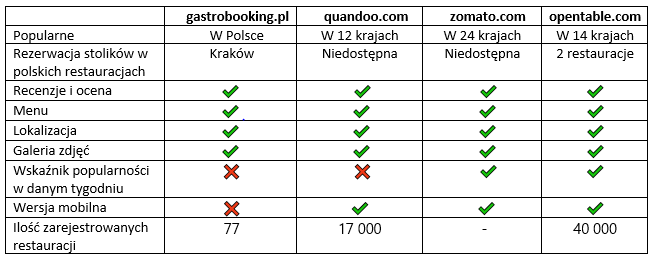
\includegraphics[width=0.95\textwidth]{konkurencjaTabela}
	\caption{Porównanie firm konkurencyjnych.}
\end{figure}

\subsubsection{Analiza wymagań biznesowych}

Wymienione w poprzednim paragrafie serwisy nie występują w Polsce, lub są słabo rozpowszechnione. W porównaniu do konkurencji podstawową zaletą aplikacji ma być jej niska cena, oraz prostota. Zwiększa to zakres firm, który mogłyby sobie pozwolić na wdrożenie naszej aplikacji, co na dłuższą metę może stanowić o większej popularności.

Główną grupą docelową naszego produktu są restauratorzy oraz obsługa restauracji z dużą liczbą rezerwacji. Dzięki przygotowanej aplikacji mogą skorzystać z najnowszych rozwiązań technicznych, aby lepiej zarządzać swoją dostępnymi miejscami, oraz personelem. Zintegrowanie opracowanego systemu z innymi systemami umożliwiającymi zarządzanie personelem, kosztami czy zamówieniami znacząco ułatwiałoby zarządzanie i podejmowanie właściwych decyzji na poziomie managerskim. 
\subsection*{Ryzyka projektu}

W projektcie przyjęto oszacowanie ryzyka na podstawie określinia poziomu ryzyka jako iloczynu prawdopodobieństwa wystąpienia i stopnia ryzyka. Wyróżniono następujące prawdopodobieństwa wystąpienia:

\begin{enumerate}
\item prakycznie niemożliwe
\item bardzo mało prawdopodobne
\item zdarza się rzadko
\item może się zdarzyć
\item duże prawdopodobieństwo zdarzenia
\end{enumerate}

Wyróżniono następujące stopnie ryzyka:

\begin{enumerate}
	\item bardzo mały
	\item mały
	\item średni
	\item duży
	\item bardzo duży
\end{enumerate}

Stosując opisaną metodykę, wybrano kila najważniejszych czynników i oszacowano poziom ryzyka.

\newpage

\begin{center}
\captionof{table}{oszacowanie poziomu ryzyka}
	\begin{tabular}{|p{4cm}|l|l|l|}
		\hline
		Ryzyko & P(w)  & Stopień ryzyka & poziom ryzyka \\ \hline
		Nie zaimplementowanie funkcji ze względu na napotkane problemy & 4 & 4 & 16 \\ \hline
		Złe oszacowanie harmonogramu projektu (diagram Gantta)  & 3 & 4 & 12 \\ \hline
		Brak współpracy w zespole , Problem z komunikacją & 4 & 4 & 16 \\ \hline
		Awaria sprzętu & 3 & 4 & 12 \\ \hline
		Zdarzenia przy projekcie (Utrata danych, złośliwe oprogramowanie , brak zasilania) & 2 & 4 & 8 \\ \hline
		Źle dobrane technologie & 2 & 4 & 8 \\ \hline
		Przekroczenie budżetu & 4 & 4 & 16 \\ \hline
		Złe decyzje projektowe podjęte na początku, mające duży wpływ na ostatnią fazę projektu i powodujące zmiany w systemie & 4 & 5 & 20 \\ \hline
		Niedostateczne zabezpieczenie danych & 4 & 4 & 16 \\ \hline
		Kłopoty związane z regulacjami prawnymi & 2 & 4 & 8 \\ \hline
\end{tabular}
\end{center}


\subsection{Wymagania funkcjonalne}

\begin{figure}
\centering
	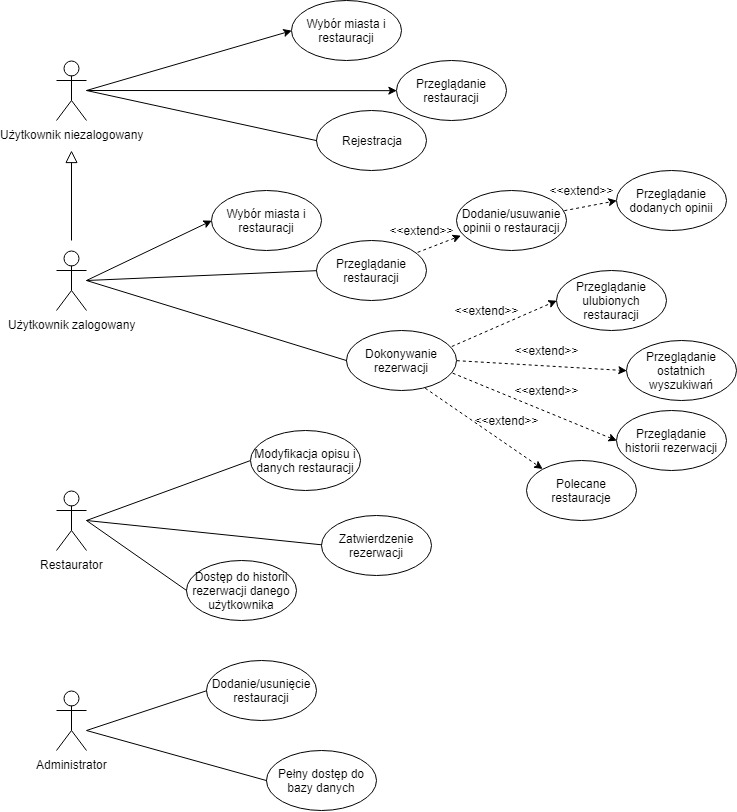
\includegraphics[width=0.90\textwidth]{use_case.jpg}
	\caption{Schemat przypadków użycia systemu.}
\end{figure}

\subsubsection{Podstawowe przypadki użycia}

Użytkowników aplikacji można podzielić na 3 grupy. Każda z grup posiada własne przypadki użycia.
\begin{enumerate}
\item klient restauracji, niezalogowany użytkownik
\begin{enumerate}
	\item przeglądanie profilu restauracji \\
	Niezalogowany użytkownik może wyświetlać profil restauracji i ma dostęp do wszystkich informacji zawartych w profilu.
	\item rejestracja \\
	Większość przypadków użycia jest dostępnych po rejestracji i zalogowaniu.
\end{enumerate}
	\item klient restauracji, zalogowany użytkownik
\begin{enumerate}
	\item złożenie rezerwacji \\
	Klient ma możliwość wyboru daty i godziny rezerwacji. Na podstawie informacji o dostępności stolików system daje informację zwrotną, czy rezerwacja w wybranych godzinach jest możliwa. Klient dokonuje rezerwacji, która następnie musi być zatwierdzona przez restaurację.
	\item dodawanie opinii o restauracji \\
	Użytkownik ma możliwość dodatnia opinii, która będzie widoczna dla wszystkich użytkowników w profilu wybranej restauracji.
	\item przeglądanie dodanych opinii \\
	Klient ma dostęp do wcześniej dodanych opinii w swoim profilu.
	\item przeglądanie ulubionych restauracji \\
	Na podstawie historii rezerwacji prezentowana jest lista ulubionych restauracji, która jest prezentowana użytkownikowi po zalogowaniu.
	\item przeglądanie historii rezerwacji \\
	Użytkownik ma dostęp do historii własnych rezerwacji.
	\item wysyłanie wiadomości do restauracji \\
	Klient może się komunikować bezpośrednio z restauracją przez stronę internetową.
	\item polecane restauracje \\
	Na postawie historii rezerwacji, oraz preferencji użytkowników o podobnych cechach prezentowana jest lista restauracji, które mogą się spodobać użytkownikowi. Do wyznaczania listy stosuje się algorytm kNN.
\end{enumerate}
\item restaurator
\begin{enumerate}
	\item zmiana informacji odnośnie restauracji \\
	Restaurator posiada możliwość zmiany danych prezentowanych na profilu restauracji. Zaliczają się do nich informacje o nazwie, adresie i zdjęcia. Restaurator nie ma wpływu na opinie widoczne na profilu jego restauracji.
	\item potwierdzenie rezerwacji \\
	Po złożeniu rezerwacji przez użytkownika, musi zostać ona zatwierdzona przez restaurację. W trakcie ewaluacji danej rezerwacji pomocne może być przeglądanie profilu klienta.
	\item wysłanie wiadomości do klienta
	Opcja bezpośredniej komunikacji przez stronę internetową.
	\item przeglądanie profilu klienta
	Restaurator ma dostęp do profilu klienta.
\end{enumerate}
\item administrator
\begin{enumerate}
	\item dodanie restauracji
	Dodawanie restauracji powinno być kontrolowane, aby uniknąć udostępniania nieprawdziwych bądź niewłaściwych informacji użytkownikom. W celu ułatwienia procesu weryfikacji danych, tylko administrator ma możliwość dodania restauracji do systemu.
	\item pełny dostęp do bazy danych
	Administrator może dodawać, usuwać, modyfikować i odczytywać wszystkie tabele w bazie. 
\end{enumerate}
\end{enumerate}


\subsection{Wymagania niefunkcjonalne}

\subsubsection{Wykorzystane technologie i narzędzia}

Projekt został zrealizowany z wykorzystaniem języka C\# oraz frameworka ASP.NET MVC. Do realizacji frontendu zostały wykorzystane HTML5, CSS 3.0 oraz JavaScript. Jako system zarządzania bazą danych wykorzystano Microsoft SQL Server.

\begin{figure}[h]
\centering
		\begin{minipage}{2cm}
			
\includegraphics[width=2cm]{c_hasztag.png}
		\end{minipage}
		\begin{minipage}{2cm}
			
\includegraphics[width=2cm]{asp_net-MVC.png}
		\end{minipage}
		\begin{minipage}{2cm}
			
\includegraphics[width=2cm]{html.png}
		\end{minipage}
		\begin{minipage}{2cm}
			
\includegraphics[width=2cm]{sql.png}
		\end{minipage}
	\caption{Wykorzystane technologie.}
	\label{fig:technologie}
\end{figure}
\begin{itemize}
\item \textbf{Język programowania C\#} \\\\
C\# jest obiektowym językiem programowania, który oficjalnie przedstawiony został w 2000 roku. Powstał na zlecenie firmy Microsoft, aby ułatwić tworzenie oprogramowania dla systemu operacyjnego Windows. W początkowej fazie swojego istnienia język był wspierany wyłącznie przez Microsoft, dlatego też rozpatrując język nieodzownym elementem było platforma programistyczna .NET. Jednak jego dobrze przemyślana struktura sprawiła, że język stał się popularny i powstało dla niego kilka open source standardów (m.in. Mono). Od 2016 roku Microsoft zmieniło swoją politykę i stworzyło .Net Core, które stało się praktycznie w pełni open source projektem. 

\item \textbf{Platforma .NET} \\\\
Do roku 2016 .NET rozwijały się dwa podejścia co do środowisk uruchomieniowych, czyli oficjalną
wersję opublikowaną przez Microsoft, jak i tworzoną przez pasjonatów wersja open source. Jednak wraz z
publikacją .NET Core 1.0 rozwój platformy został połączony w jedno. Wprowadzono ujednolicony standard
platformy (.NET Standard Library). Dzięki temu tworzone od teraz biblioteki są możliwe w użyciu również dla .NET Core, Xamarin i .NET Framework. Platforma .NET wspiera nie tylko język C\# ale również takie języki jak m.in. F\#, Visual Basic, C++. .NET Framework udostępnia specyficzne dla systemu operacyjnego Windows API takie jak Windows Forms i WPF (tworzenie aplikacji okienkowych). .NET Core zakłada całkiem odmienne podejście do przeznaczenia od wcześniejszego standardu. Głównym
założeniem jest wieloplatformowość. Przykładem API są: ASP.NET Core (aplikacje webowe) oraz Universal Windows Platform (docelowo reużywalne oprogramowanie działające zarówno na komputerach, urządzeniach mobilnych, jak i dla aplikacji wspierający Internetu rzeczy itd.). Mono for Xamarin w tej chwili wersja .NET dla aplikacji działających pod iOS oraz Android. Historycznie opensource’owa wersja standardu .NET Framework.
\item \textbf{ASP.NET Core 2.0} \\\\
ASP.NET to API umożliwiające tworzenie aplikacji webowych\cite{asp}, czyli takie, które do swojego działania potrzebują jedynie przeglądarki internetowej. Nie wymagają od użytkownika instalowania zewnętrznego oprogramowania. Dzięki temu stworzone aplikację działają na wielu platformach jednocześnie. Dodatkowo wszelkie zmiany wprowadzane są wyłącznie po stronie serwera (nie angażują użytkownika). Do głównych elementów API zaliczamy: Web Forms, MVC (MVC + Web Page + Web API) oraz SignalR. Wprowadzenie standardu .NET Core uporządkowało kwestie związane z różnym podejściem tworzenia aplikacji webowych. Web Forms oraz Web Page praktycznie przestały istnieć.

\item \textbf{Entity Framework Core} \\\\
Entity Framework Core to narzędzie pozwalające przetłumaczyć relacyjne bazy danych na obiekty. Narzędzia
te nazywamy ORM (Object Relational Mapping). Dzięki temu podejściu można tworzyć bazy danych bez użycia języka SQL. Ułatwia to zarządzanie danymi oraz przyspiesza pracę z nimi. Ponadto biblioteka ta zapewnia wsparcie nie tylko na poziomie tworzenia zapytań, ale również dzięki podejściu Code First możemy zaprojektować relacyjną bazę danych z poziomu języka obiektowego. Entity Framework pozwala także tworzyć automatycznie obiekty na podstawie już istniejącej bazy. Ostatnim wspieranym podejściem jest tworzenie bazy przy pomocy podejście Model first polegające na stworzeniu modelu w ADO.NET Entity Data Model Designer, a następnie Entity Framework tłumaczy go na obiekty oraz relacyjną bazę danych.

\item \textbf{Bootstrap} \\\\
Biblioteka zapewniająca głównie style CSS, ale również określa ich zachowanie (wykorzystuje JavaScript). Główną zaletą Bootstrap jest to, że wspomaga tworzenie responsywnych aplikacji webowych, to znaczy, że powinny dobrze wyglądać nie tylko na monitorze, ale również na tablecie, czy telefonie komórkowym. Pomaga w kontrolowaniu zachowania gotowych komponentów HTML.

\item \textbf{jQuery} \\\\
JQuery jest biblioteką JavaScript ułatwiająca manipulacją drzewa DOM (Document Object Mode).
Wykorzystanie jQuery eliminuję problem interpretacji kodu JS przez różne przeglądarki. Jego niewątpliwą
zaletą jest wbudowanie AJAX. Sprawia, że opisane rozwiązanie jest czytelniejsze oraz wprowadza uproszczone
odwołanie się do elementów strony, oraz wykorzystania AJAX.

\item \textbf{SignalR} \\\\
SignalR jest biblioteką Microsoft ASP.NET, która pozwala na wysyłanie asynchronicznych powiadomień do aplikacji po stronie klienta. Biblioteka zawiera komponenty JavaScript po stronie serwera i po stronie klienta. Umożliwia dodanie funkcjonalności do aplikacji w czasie rzeczywistym. 
\end{itemize}


\section{Projekt systemu}

\subsection{Architektura systemu} \label{Architektura systemu}

W niniejszym rozdziale przedstawiono ogólny przegląd architektury całej aplikacji, opartej na zalecanych sposobach pracy z wybranymi narzędziami.

\subsubsection{ASP.NET MVC}

Projekty wykonywane w frameworku ASP.NET MVC wymuszają pewną organizację projektu, która zwiększa uporządkowanie oraz wymusza korzystanie z dobrych praktyk. W projekcie można wyróżnić 4 zasadnicze części: Views, Controllers, Models i Router. Poniżej przedstawiono krótki opis poszczególnych części.

\paragraph{Model}
Modele są odpowiedzialne za przechowywanie informacji domenowej i stanu aplikacji. Najczęściej są implementowane jako Plain Old CLR Object (POCO) i służą do modelowania danych z bazy. Obiekty te są niezależne od frameworków, systemu zarządzania bazą danych czy mapowań ORM. Modele mogą być łączone w ViewModele, aby ułatwić grupowanie i przekazywanie informacji w aplikacji.

\paragraph{View}
Jest to frontendowa część projektu, która determinuje wygląd strony pokazywanej użytkownikowi. Technologie wykorzystywane w tym obszarze to HTML, CSS oraz JavaScript. Dodatkowo do widoku są przesyłane dane z innych komponentów w postaci modeli lub viewmodeli. ASP.NET MVC umożliwia dodawanie fragmentów kodu w C\# do ułatwienia wykorzystywania danych z modeli.

\paragraph{Controler}
Najczęściej jest to element implementujący wybraną część logiki biznesowej. Wykorzystuje dane z Modeli, aby wytworzyć i przekierować użytkownika do odpowiedniego Widoku. Każdy controler jest odpowiedzialny za obsługę HTTP Request. Taka organizacja wymusza podział projektu na mniejsze klasy z dobrze zdefiniowanym zakresem odpowiedzialności.

\paragraph{Router}
Jest to komponent, który odpowiada za mapowanie zapytań HTTP na poszczególne akcje w kontrolerach.
\\\\
Pierwsze trzy komponenty są dobrze znane ze wzorca projektowego na Model-View-Controler, natomiast ostatni jest często spotykanym dodatkiem w wielu frameworkach sieciowych, umożliwiający łatwe mapowanie. Konstrukcja frameworku MVC pozwala na łatwe rozdzielenie odpowiedzialności komponentów i klas oraz wstrzykiwanie zależności do poszczególnych klas.

\subsubsection{Architektura warstwowa}

Wzorzec programowania oparty na architekturze warstwowej (ang. tier architectrue) jest powszechny w procesie tworzenia aplikacji internetowych. Podejście te rozdziela logikę systemu od interfejsu użytkownika. W podejściu architektury trzywarstwowej wyróżniamy następujące warstwy:

\begin{figure}[h]
\centering
	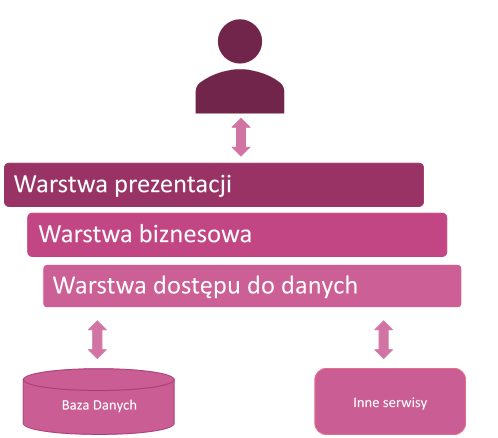
\includegraphics[width=0.50\textwidth]{ntier.png}
	\caption[caption]{Warstwy w architekturze wielowarstwowej.}
	\label{fig:tier}
\end{figure}

\begin{itemize}
\item \textbf{Warstwa prezentacji (ang. presentation tier)} - odpowiedzialna za przedstawienie funkcjonalności użytkownikowi, umożliwiająca wyświetlanie oraz wprowadzanie danych. W tej warstwie ASP.NET używa się oprócz języka platformy (np. C\#) języków do opisów wyglądu strony (CSS, HTML, JavaScript). 
\item \textbf{Warstwa biznesowa (ang. business tier)} - w miejscu tym umieszczona jest logika aplikacji. Dane pozyskane z warstwy danych są przetwarzane by były w odpowiedni sposób przygotowane do wysyłania do warstwy prezentacji, jak również pozyskane od użytkownika przekształcane są w oczekiwanej formie, transportowane są do warstwy danych.

\item \textbf{Warstwa danych (ang. persistance tier)} - odpowiedzialna za komunikacji z zewnętrznymi serwisami zarządzającymi danymi, np. z bazą danych.
\end{itemize}

Dzięki zastosowaniu tego podejściu zyskujemy łatwość modyfikacji poszczególnych funkcjonalności, ponieważ zmiana w jednej warstwie nie wymusza zmian w całym systemie. Inną zaletą jest fakt, iż tworzone rozwiązania stają się bardziej przejrzyste. Za używaniem tego sposobu projektowania aplikacji przemawia to, że tę samą logikę możemy wykorzystać zarówno przy tworzeniu aplikacji internetowych jak i mobilnych. Wykorzystanie architektury warstwowej pozwala na reużywalność zaimplementowanych komponentów oraz ogranicza liczbę błędów (poprzez użycie wstrzykiwania zależności lub interfejsów), poza bieżącą warstwą nie ma dostępu do wewnętrznych metod. W stworzonym systemie oprócz przedstawionego podziału wprowadzono dodatkowy element przytrzymujący modele wykorzystywane między warstwami. Ich szczególnym przykładem są modele DAO, które używane są wyłącznie przez warstwę danych do komunikacji z bazą danych (mapowane są one przy użyciu Automappera). Dla realizacji założeń każda warstwa zaimplementowana została w osobnym projekcie.

\subsection{Diagram elementów systemu}

\begin{figure}[H]
\centering
	\includegraphics[width=1.00\textwidth]{system.png}
	\caption[caption]{Diagram elementów systemu.}
	\label{fig:system}
\end{figure}

Zgodnie z przyjętą architekturą kod projektu można podzielić na cztery części: Widoki, Kontrolery, Serwisy, oraz Repozytoria. Odpowiedzialności poszczególnych części opisano w rozdziale \ref{Architektura systemu}. Kontrolery uzyskują dostęp do Serwisów poprzez wstrzykiwanie zależności. Ten sam mechanizm wykorzystano przy zapewnieniu dostępu serwisom do Repozytoriów. Poprzez wizualną analizę diagramu \ref{fig:system} można wyróżnić elementy systemu wymagające poprawy. Definitywnie pierwszym kandydatem do procesu refactoryzacji kodu jest ReservationService. Wnioskując po ilości powiązań z Repozytoriami klasa ta ma zbyt dużą odpowiedzialność i powinna zostać podzielona na mniejsze komponenty. Podobne wnioski można wyciągnąć na temat RestaurantService. Mimo tych niedoskonałości przy implementacji systemu zachowano warstwową architekturę.

\subsection{Projekt frontendu}

\begin{figure}[H]
\centering
	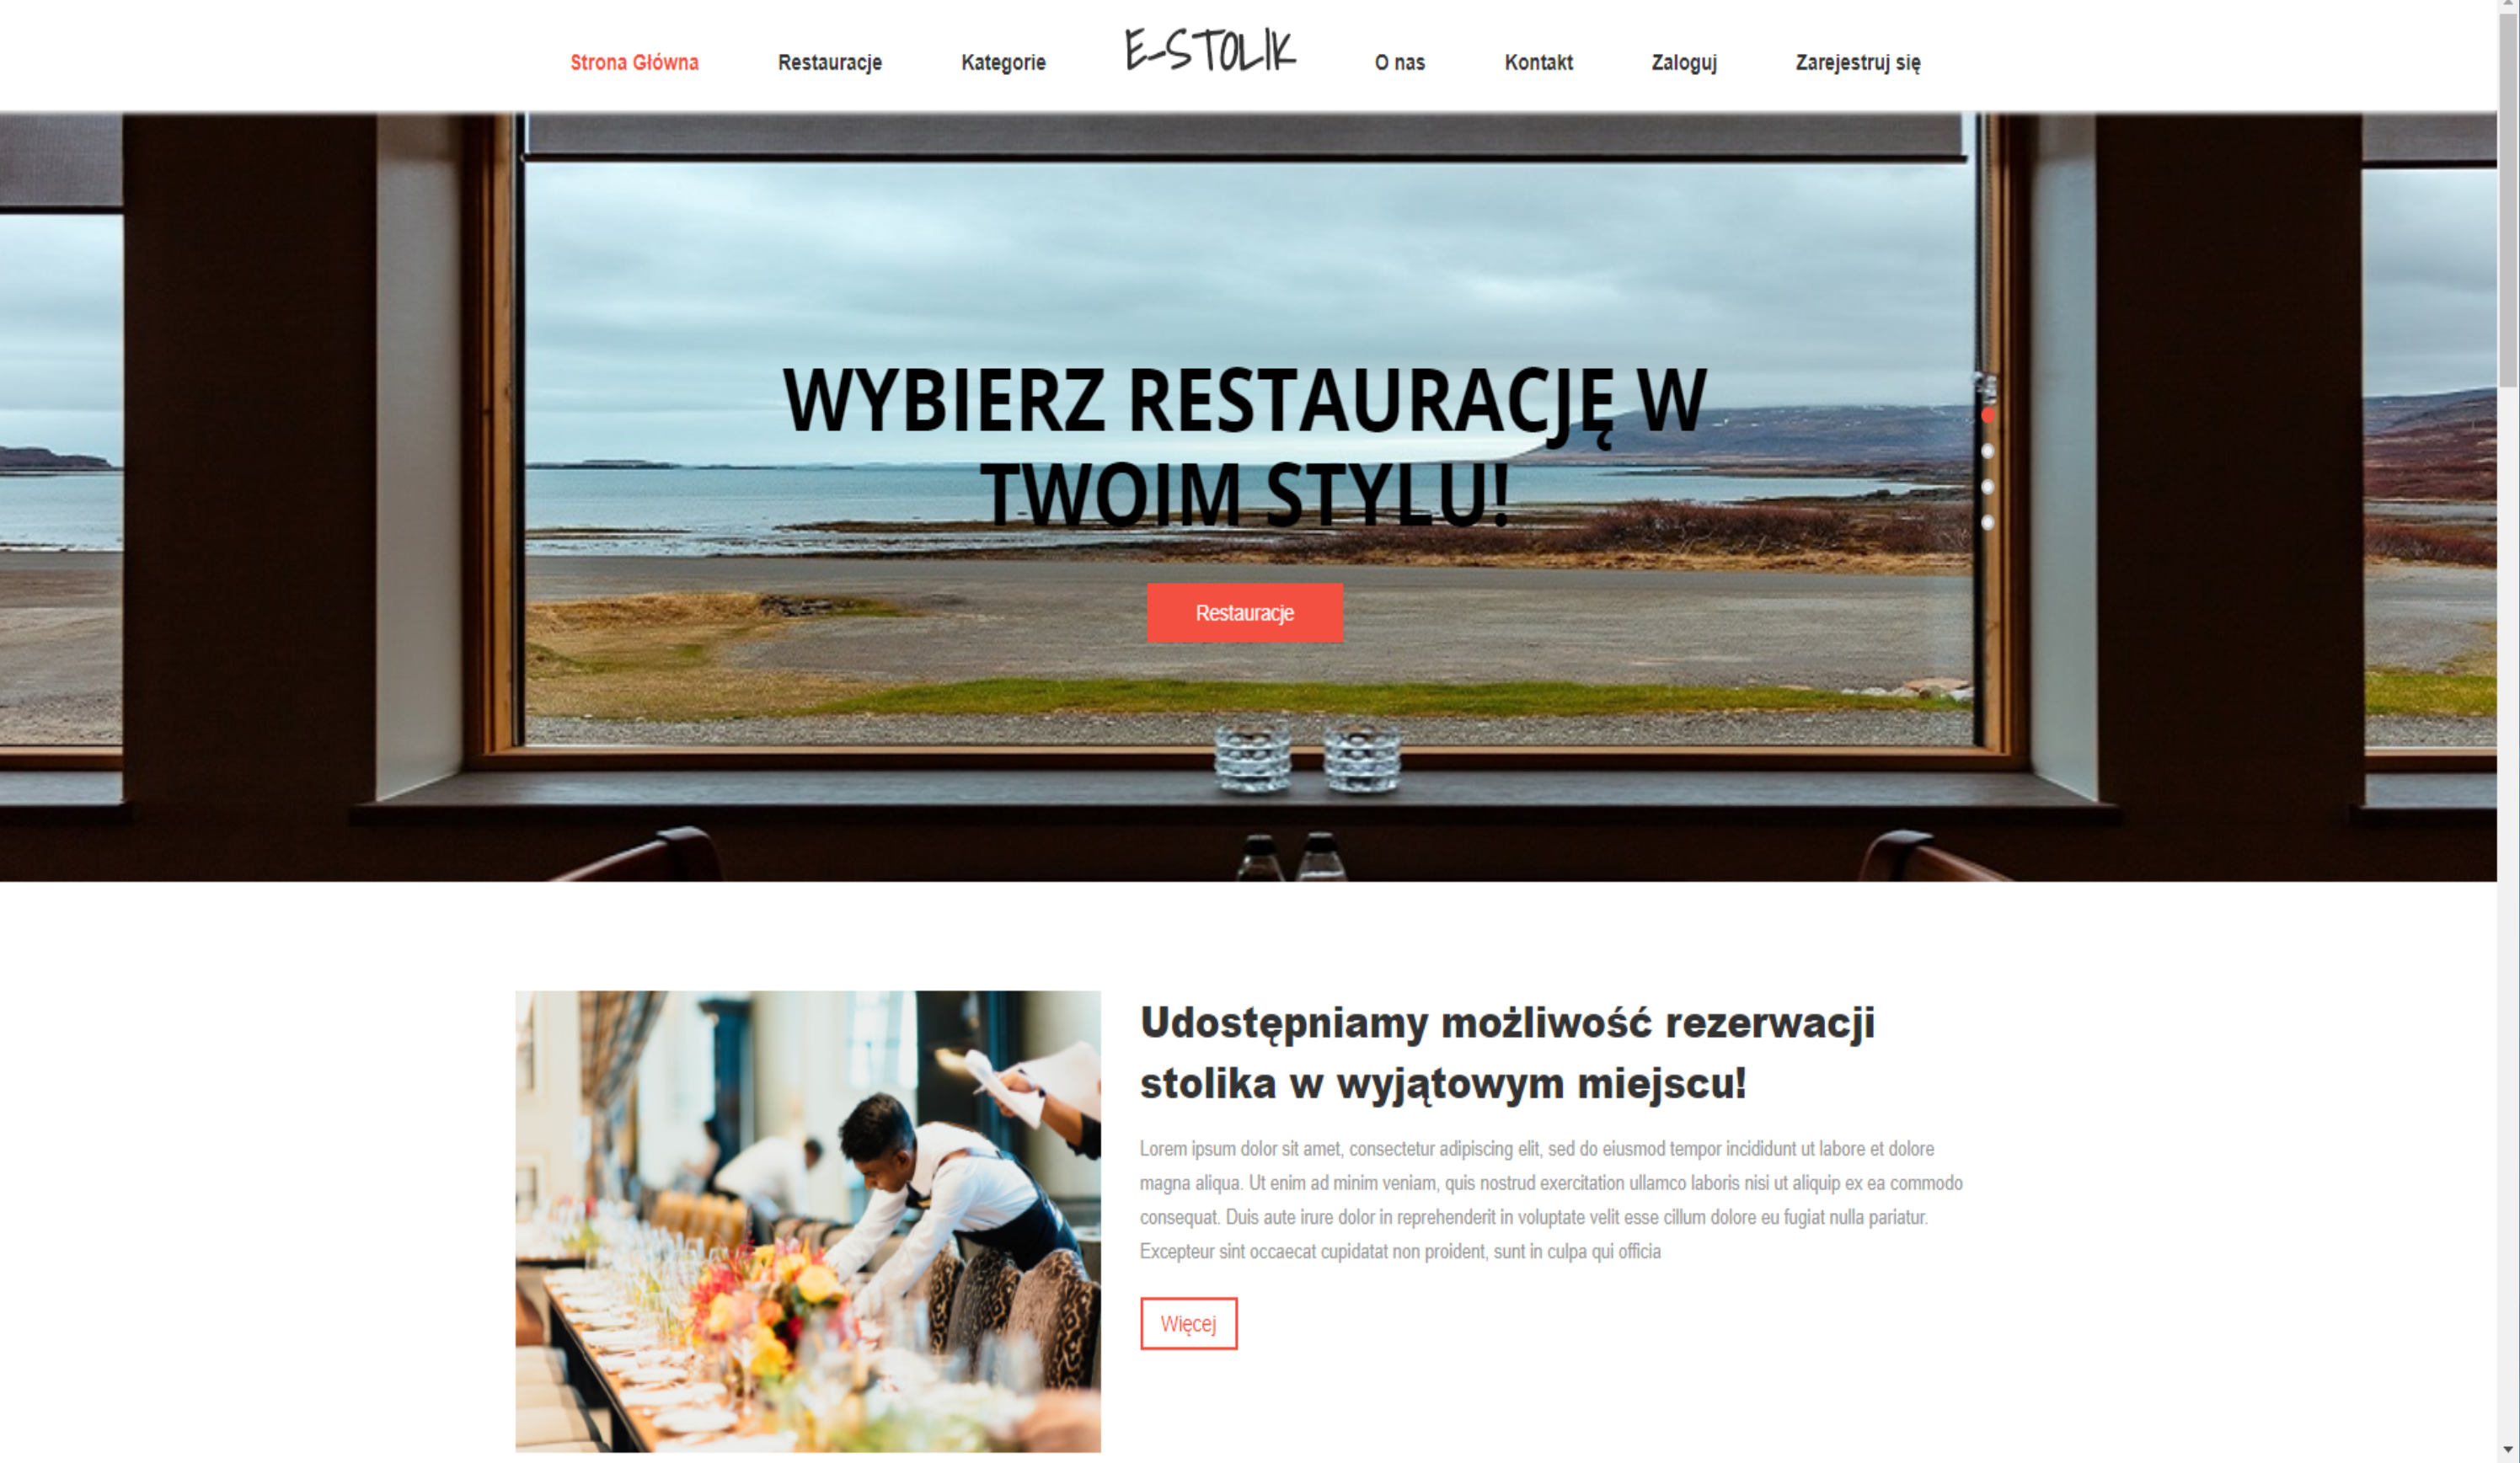
\includegraphics[width=1.00\textwidth]{screens/index1.png}
	\caption[caption]{Widok strony głównej.}
	\label{fig:index}
\end{figure}

\begin{figure}[H]
\centering
	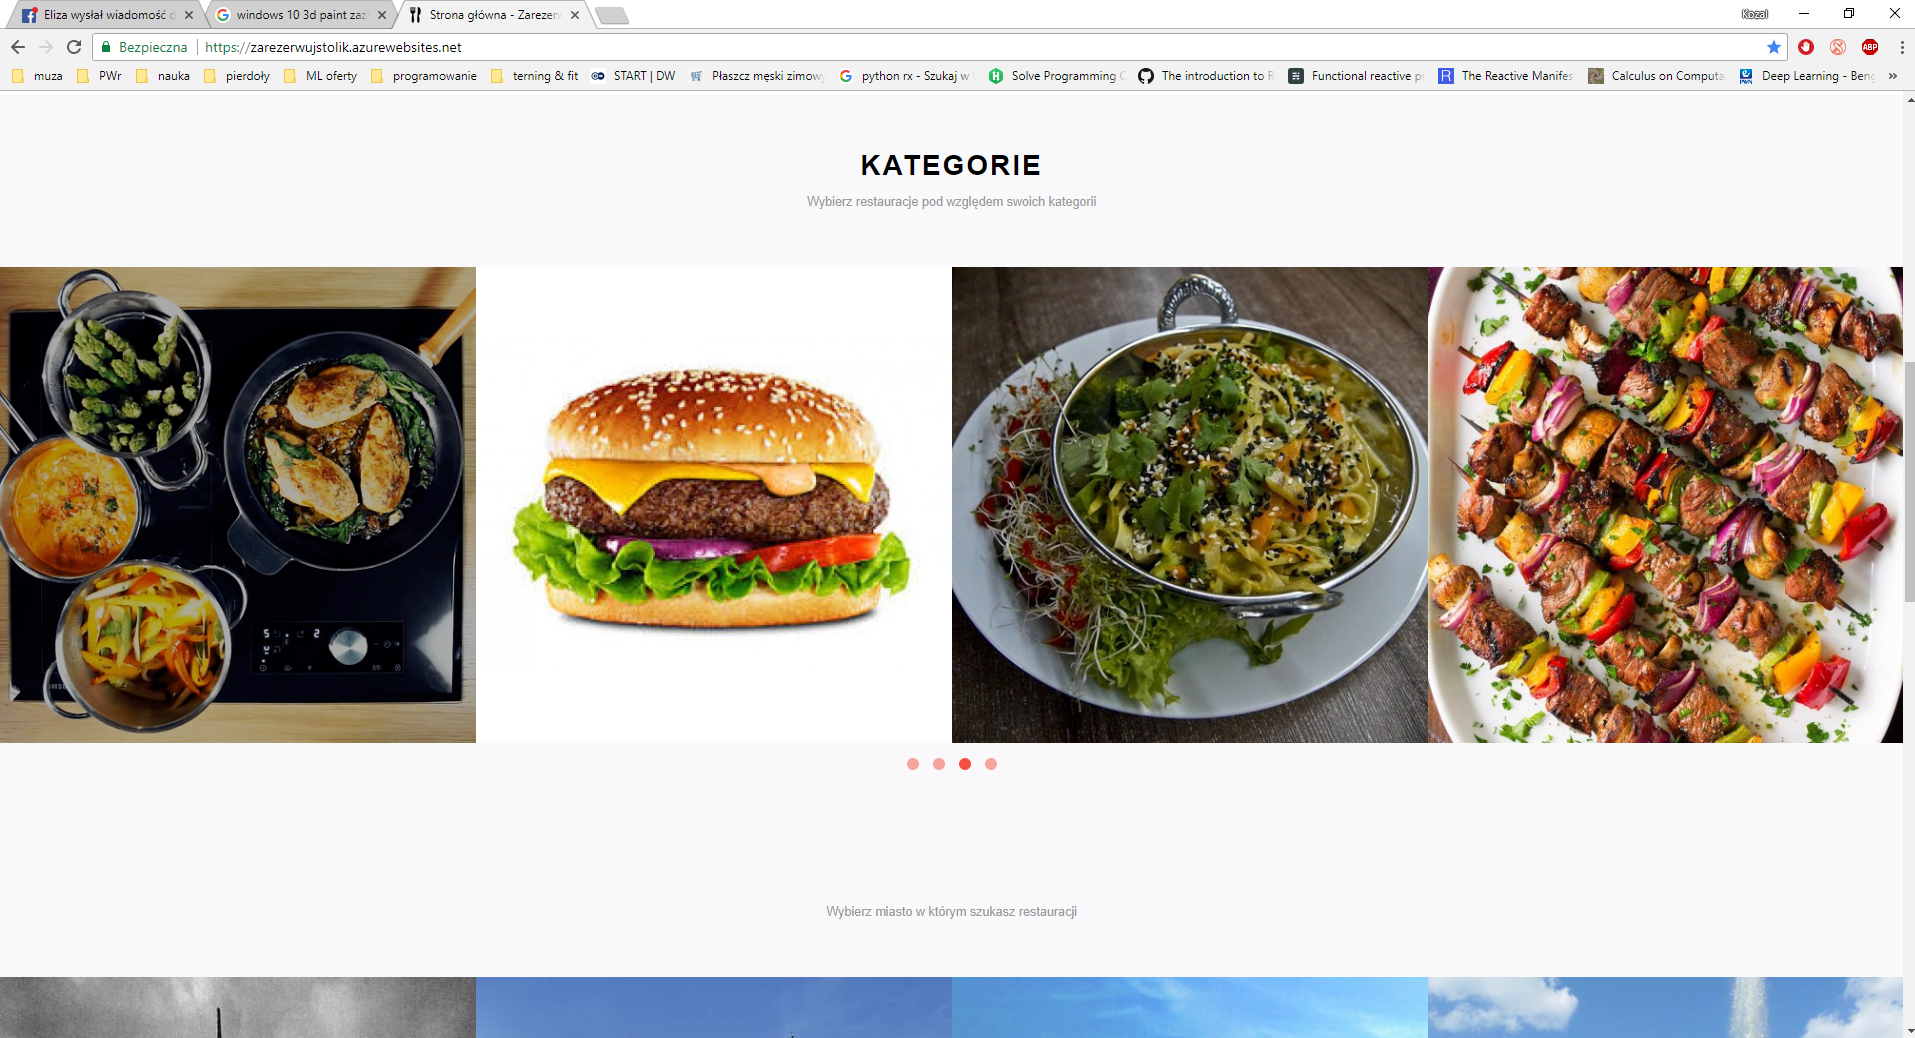
\includegraphics[width=1.00\textwidth]{screens/index2.png}
	\caption[caption]{Widok kategorii na stronie głównej.}
	\label{fig:index_category}
\end{figure}

\begin{figure}[H]
\centering
	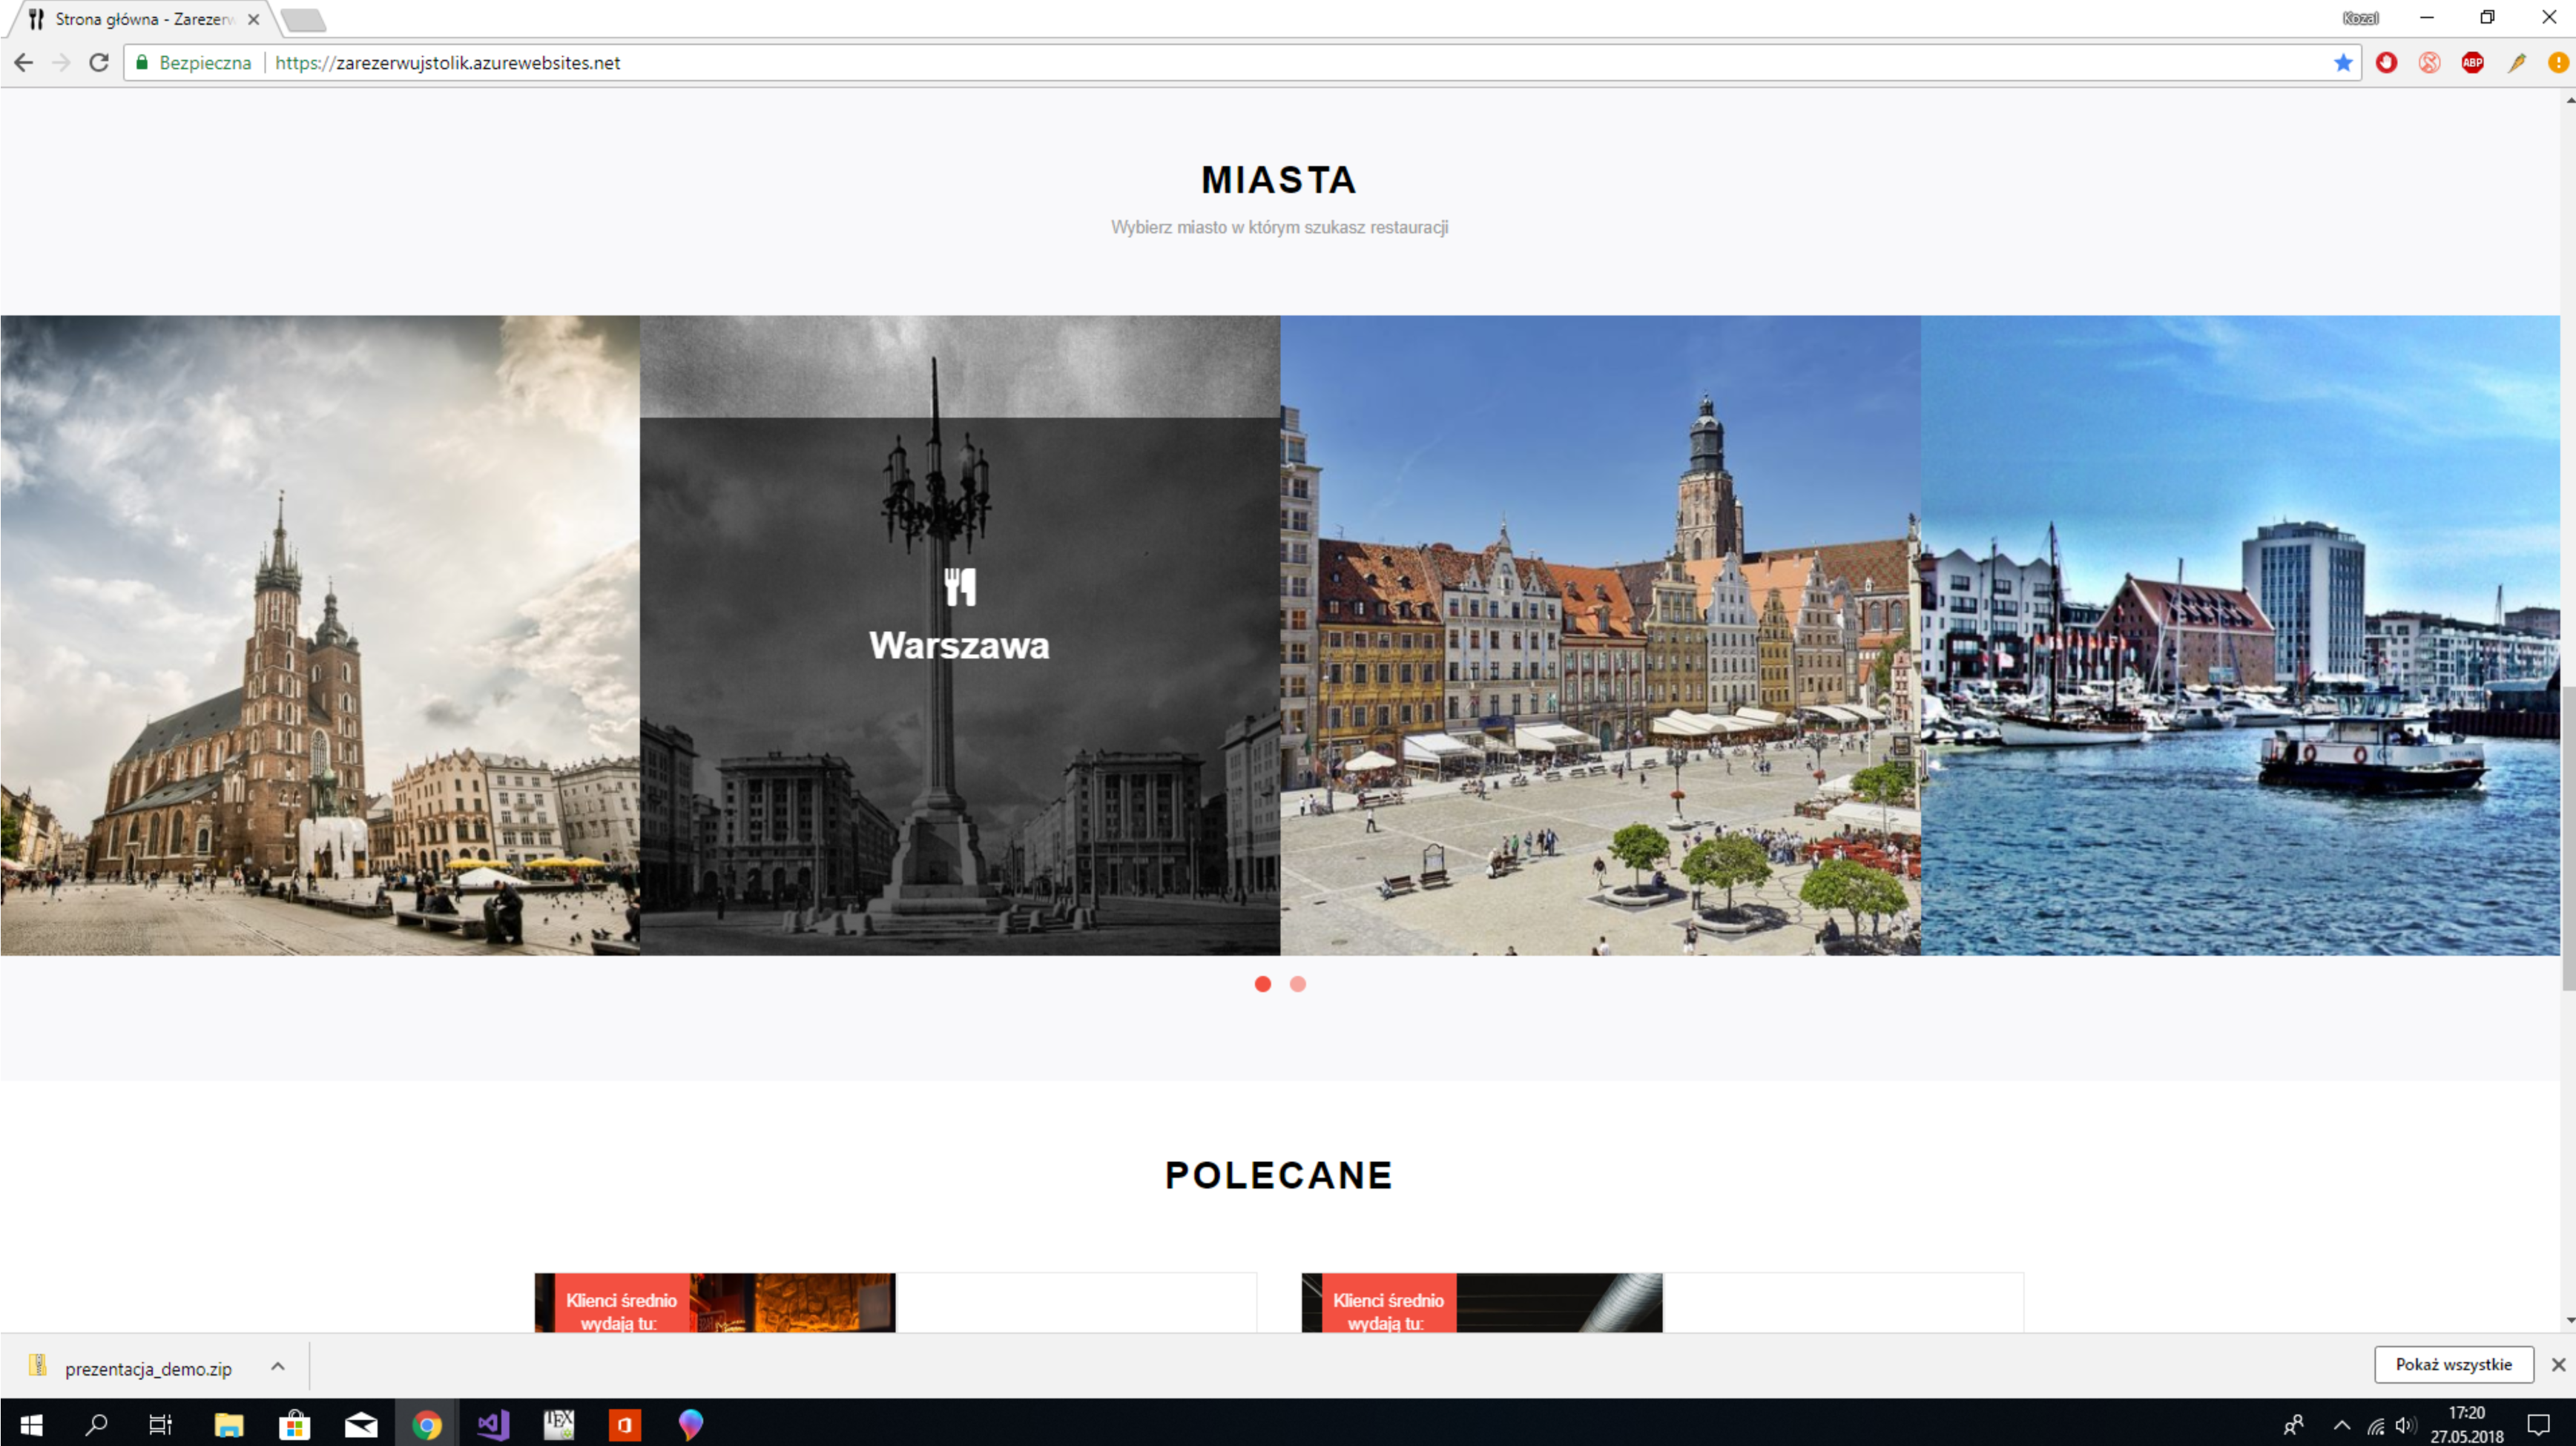
\includegraphics[width=1.00\textwidth]{screens/index3.png}
	\caption[caption]{Widok miast na stronie głównej.}
	\label{fig:index_cities}
\end{figure}

\begin{figure}[H]
\centering
	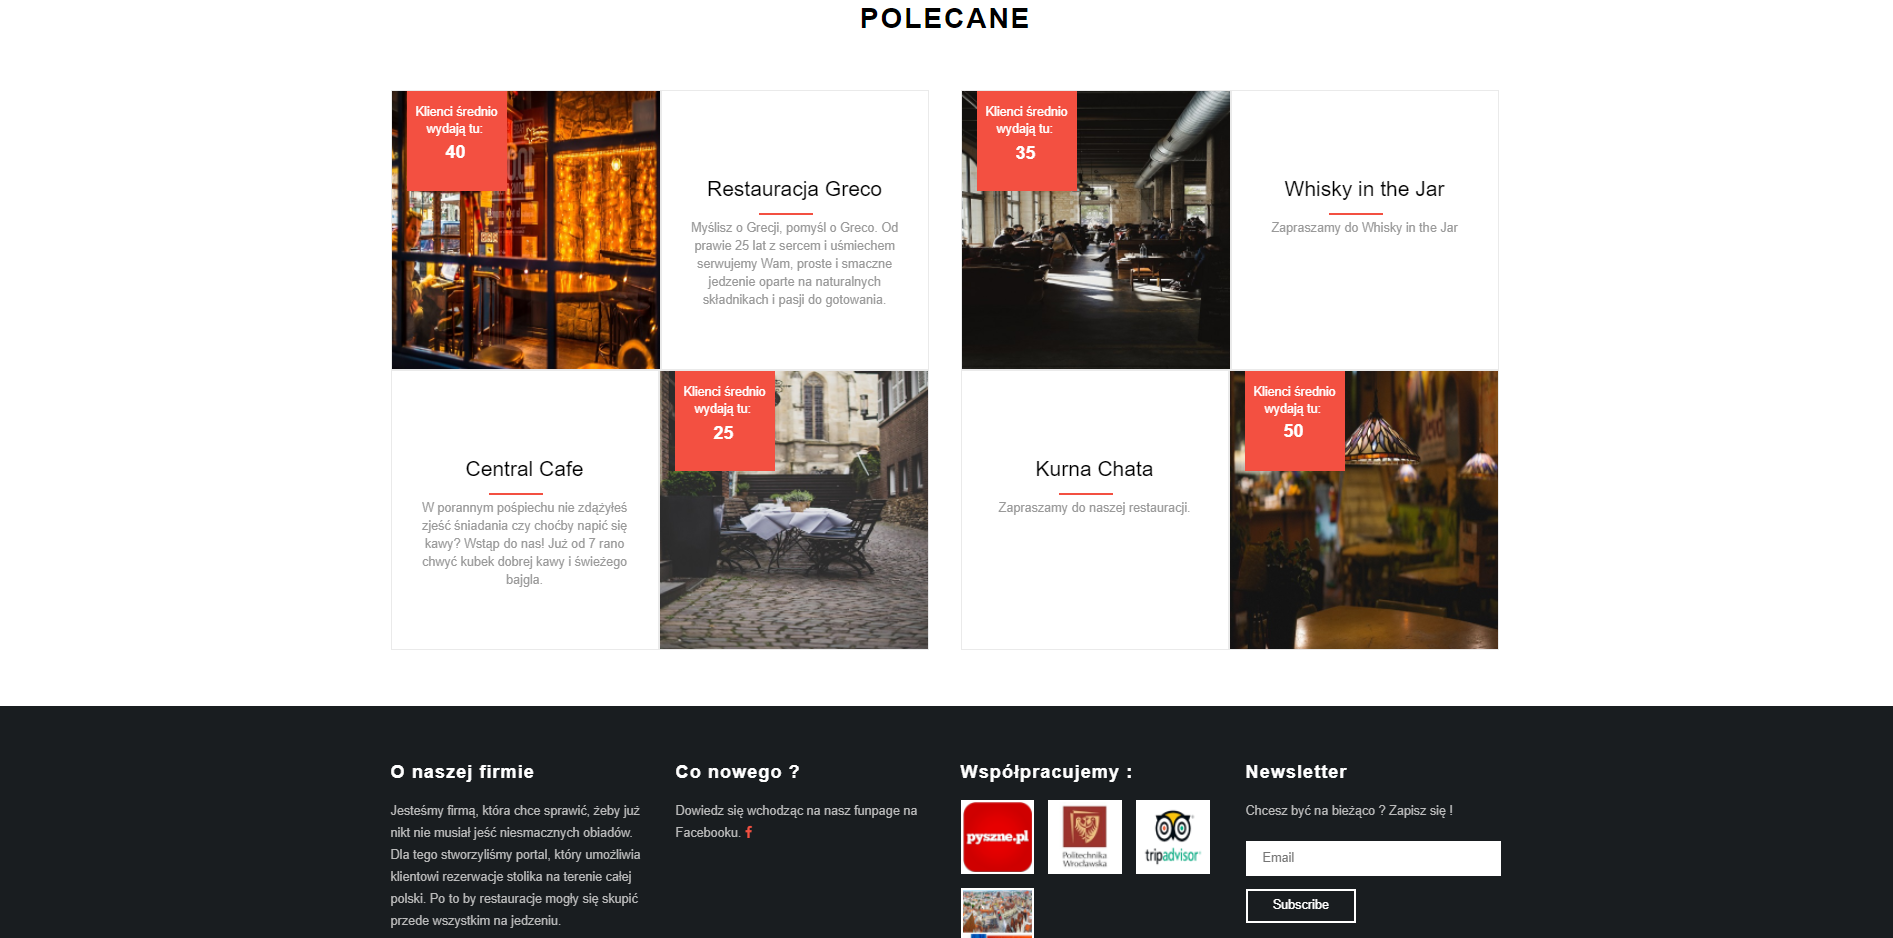
\includegraphics[width=1.00\textwidth]{screens/index4.png}
	\caption[caption]{Widok polecanych restauracji.}
	\label{fig:index_recomended}
\end{figure}

Na stronie głównej znajdziemy odnośniki do wszystkich części systemu. Pasek nawigacyjny u góry strony pozwala na przełączanie się między widokami i łatwe poruszanie się po stronie. Jest on dostępny we wszystkich widokach w systemie. Widok strony głównej (rys. \ref{fig:index}-\ref{fig:index_recomended}) zawiera informacje na temat dostępnych kategorii, miast oraz polecanych restauracji. Po wybraniu jednej z kategorii (rys. \ref{fig:index_category}) użytkownik jest przekierowany do widoku zawierającego listę restauracji z wybraną kategorią. Analogicznie, po wybraniu miasta (rys. \ref{fig:index_cities}) użytkownik jest przkierowywany do widoku zawierającego listę restauracji w wybranym mieście. Sekcja polecane zawiera listę rekomendowanych restauracji po wybraniu, użytkownik jest przekierowywany do widoku ze szczegółami rezerwacji.

\begin{figure}[H]
\centering
	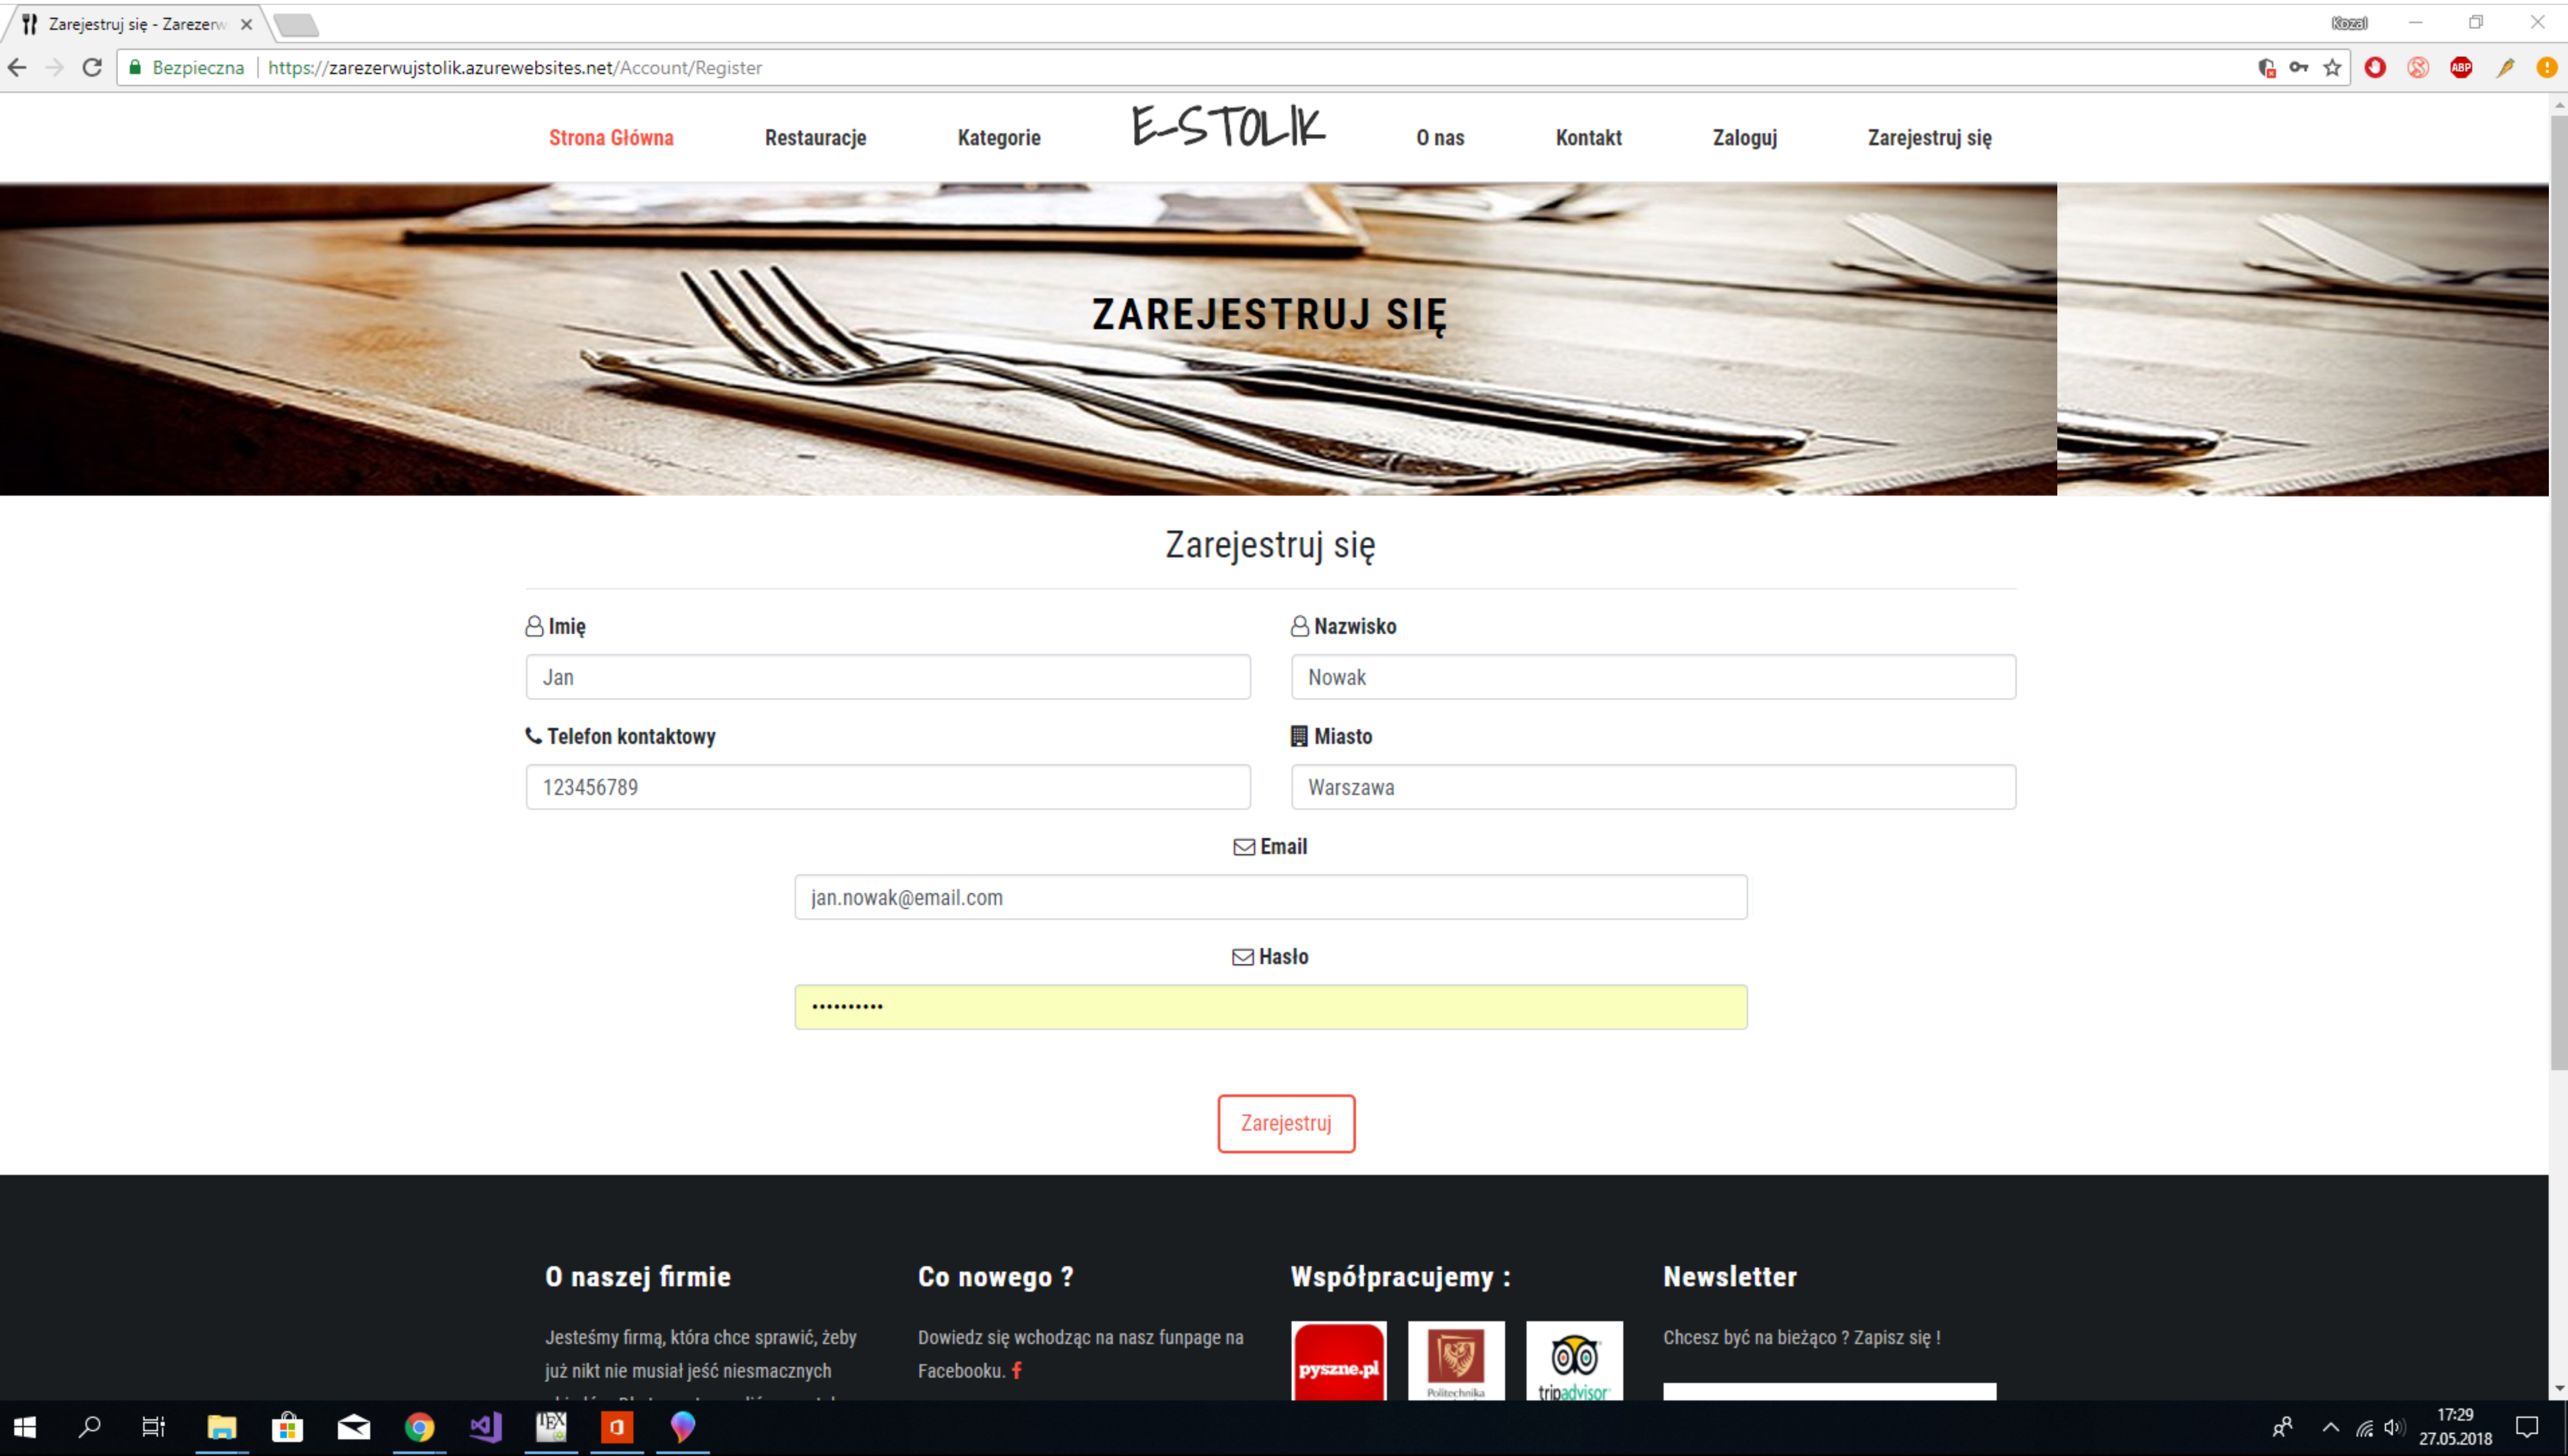
\includegraphics[width=1.00\textwidth]{screens/register.png}
	\caption[caption]{Widok rejestracji.}
	\label{fig:register}
\end{figure}

\begin{figure}[H]
\centering
	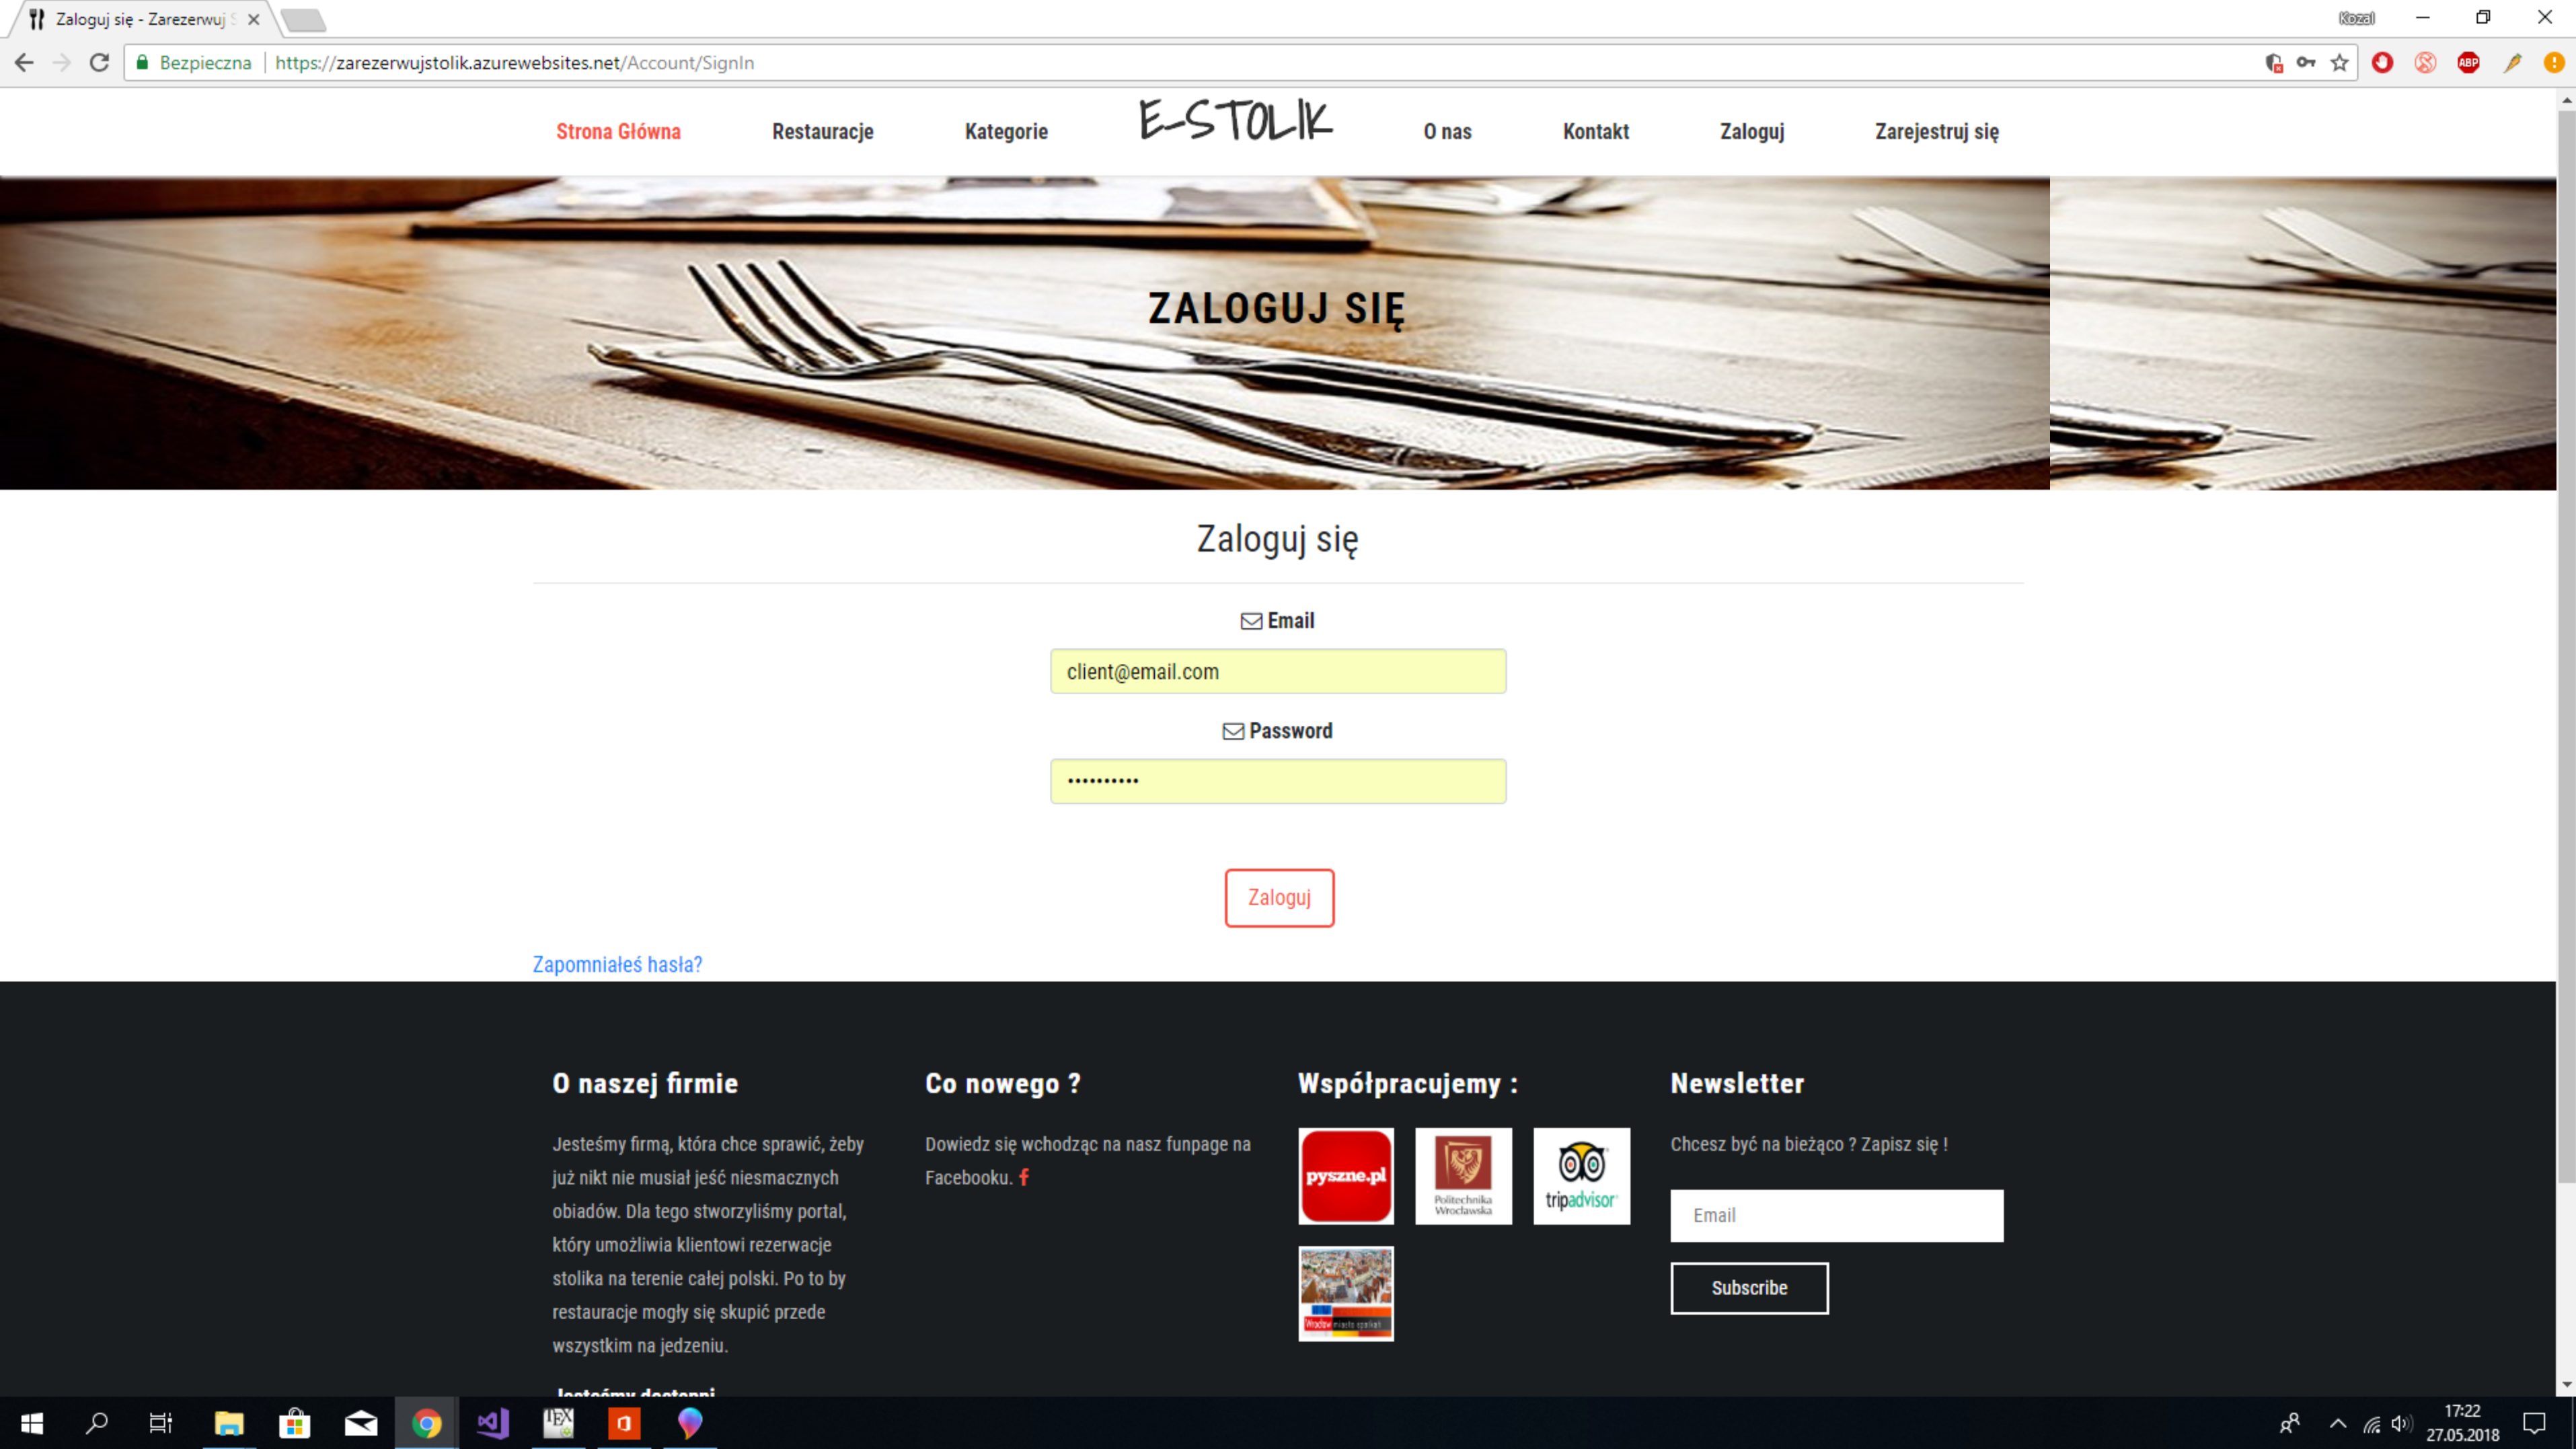
\includegraphics[width=1.00\textwidth]{screens/login.png}
	\caption[caption]{Widok logowania.}
	\label{fig:login}
\end{figure}

\begin{figure}[H]
\centering
	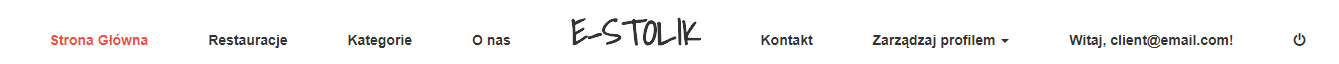
\includegraphics[width=1.00\textwidth]{screens/loged_in.png}
	\caption[caption]{Pasek nawigacyjny po zalogowaniu.}
	\label{fig:loged_in}
\end{figure}

Aby uzyskać możliwość rezerwowania stolików klient musi być zalogowany. W tym celu należy się zalogować (widok na rys. \ref{fig:login}) lub zarejestrować (widok na rys. \ref{fig:register}). Po zalogowaniu fakt nazwa użytkownika będzie widoczna zamiast przycisku zaloguj na pasku nawigacyjnym (rys. \ref{fig:loged_in}).

\begin{figure}[H]
\centering
	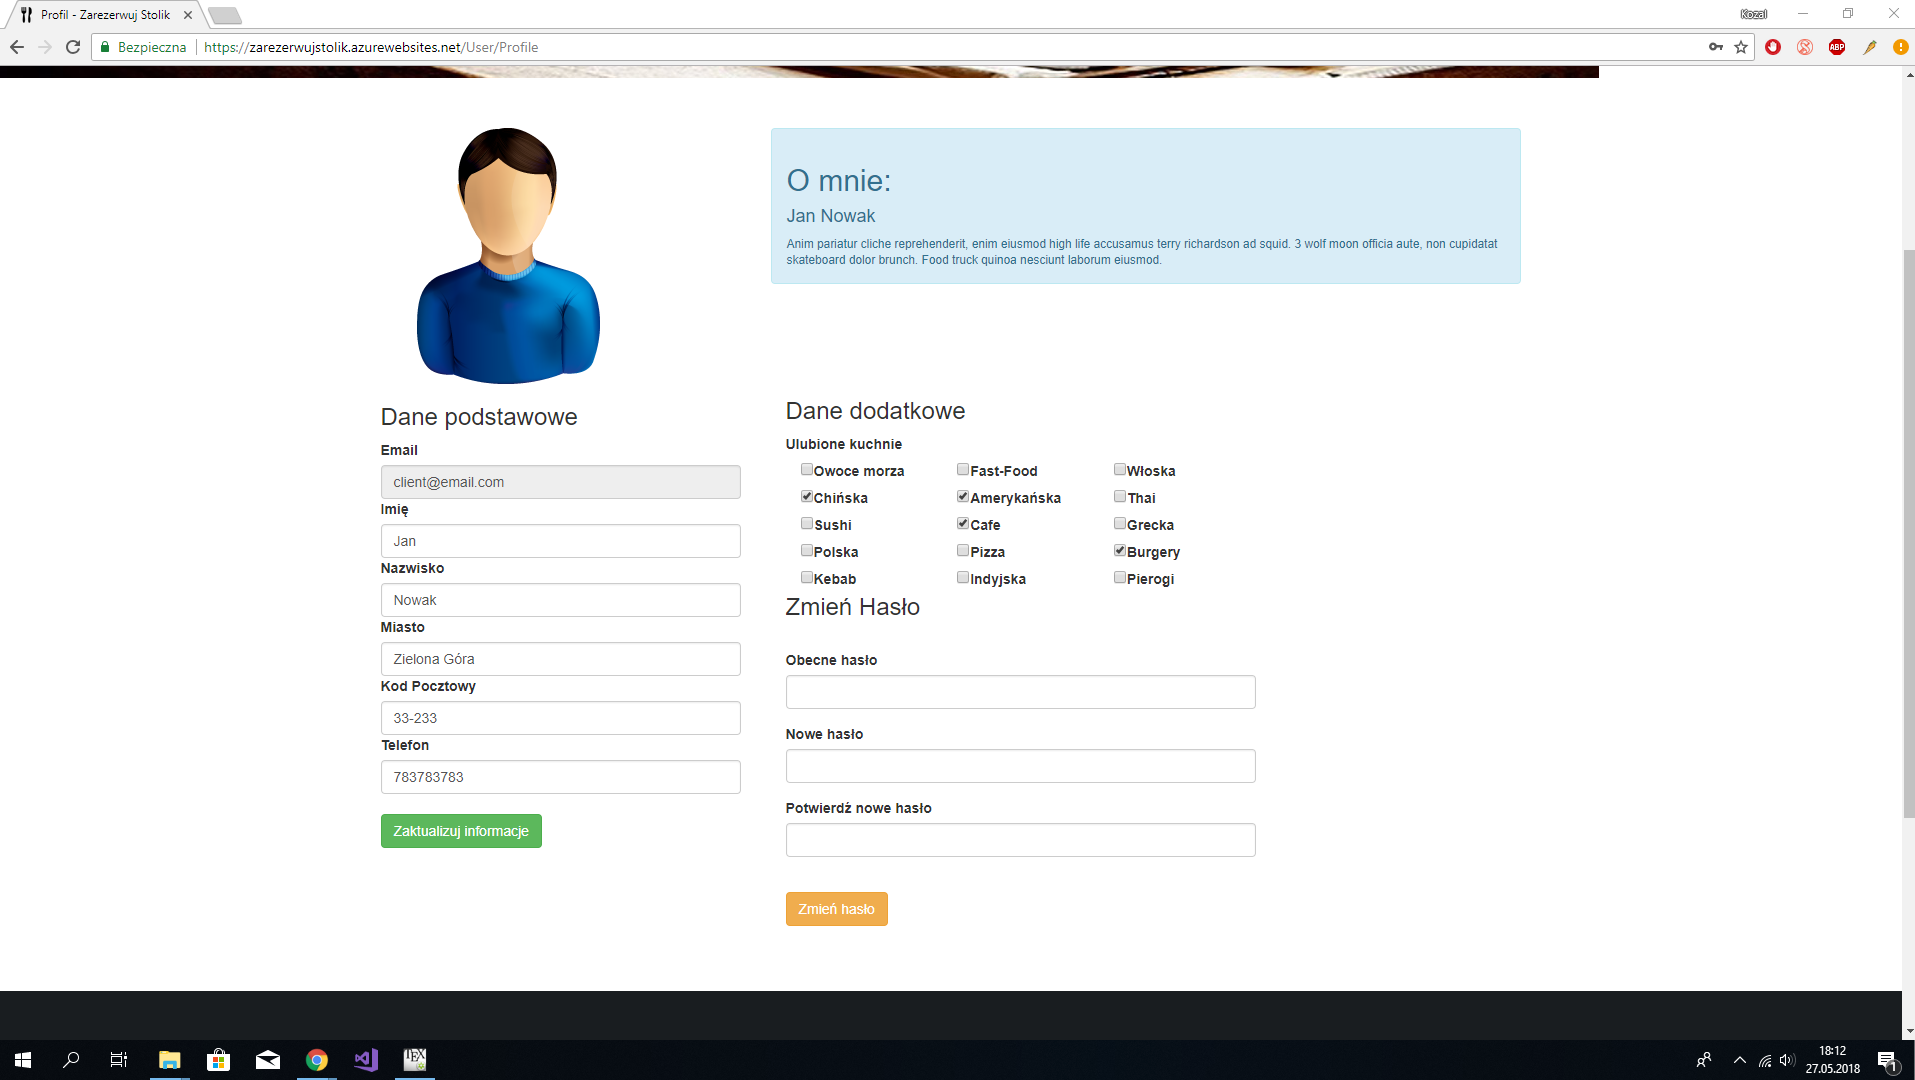
\includegraphics[width=1.00\textwidth]{screens/account_profile.png}
	\caption[caption]{Widok szczegółów konta użytkownika.}
	\label{fig:account_details}
\end{figure}

Po zalogowaniu użytkownik może przeglądać szczegóły swoje konta. W pasku nawigacyjnym należy wybrać "Zarządzaj profilem" a następnie z listy wysuwanej "Mój profil", aby zyskać dostęp do danych osobowych, oraz wyboru ulubionych kategorii. W tym samym widoku znajduje się równiej opcja zmiany hasła (rys. \ref{fig:account_details}).

\begin{figure}[H]
\centering
	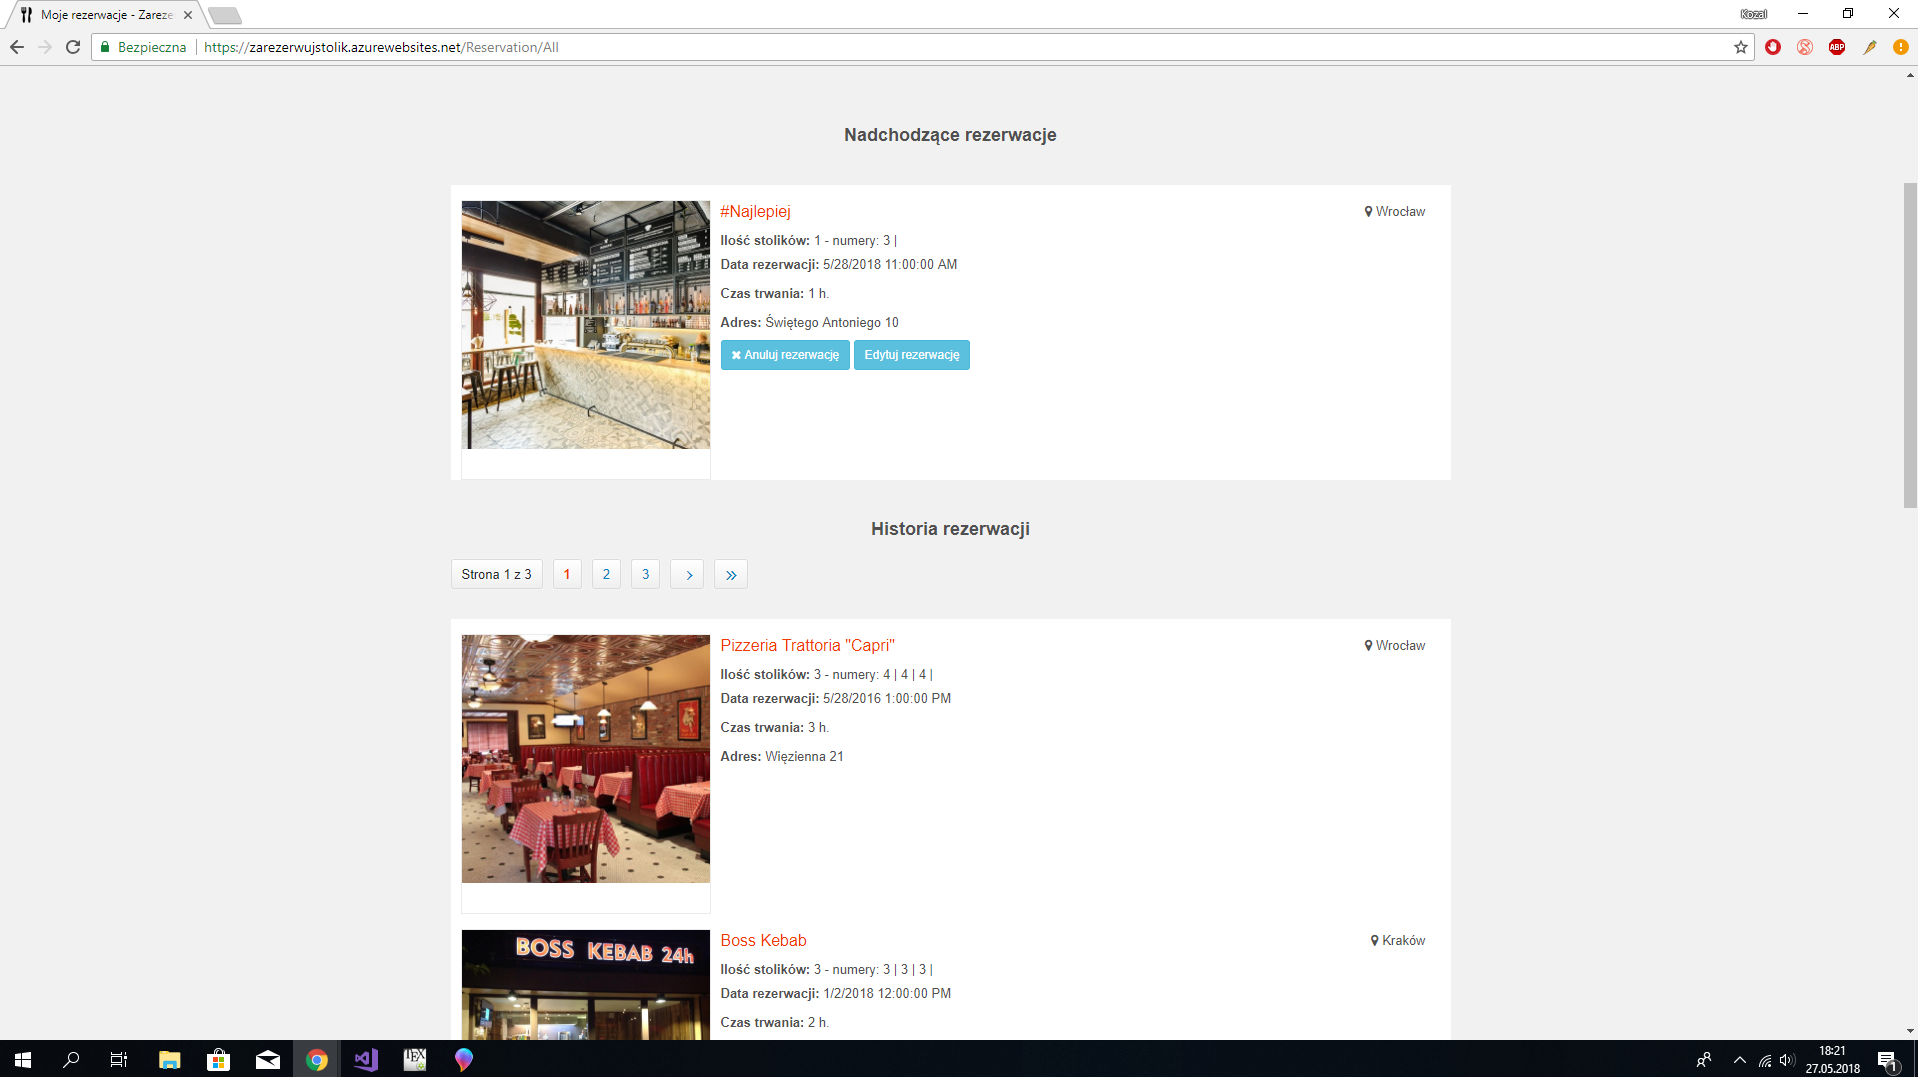
\includegraphics[width=1.00\textwidth]{screens/reservations_history.png}
	\caption[caption]{Widok historii rezerwacji.}
	\label{fig:account_reservations_history}
\end{figure}

Po wybraniu "Zarządzaj profilem" oraz "Moje rezerwacje" użytkownik może przeglądać nadchodzące rezerwacje oraz historie rezerwacji (rys. \ref{fig:account_reservations_history}).

\begin{figure}[H]
\centering
	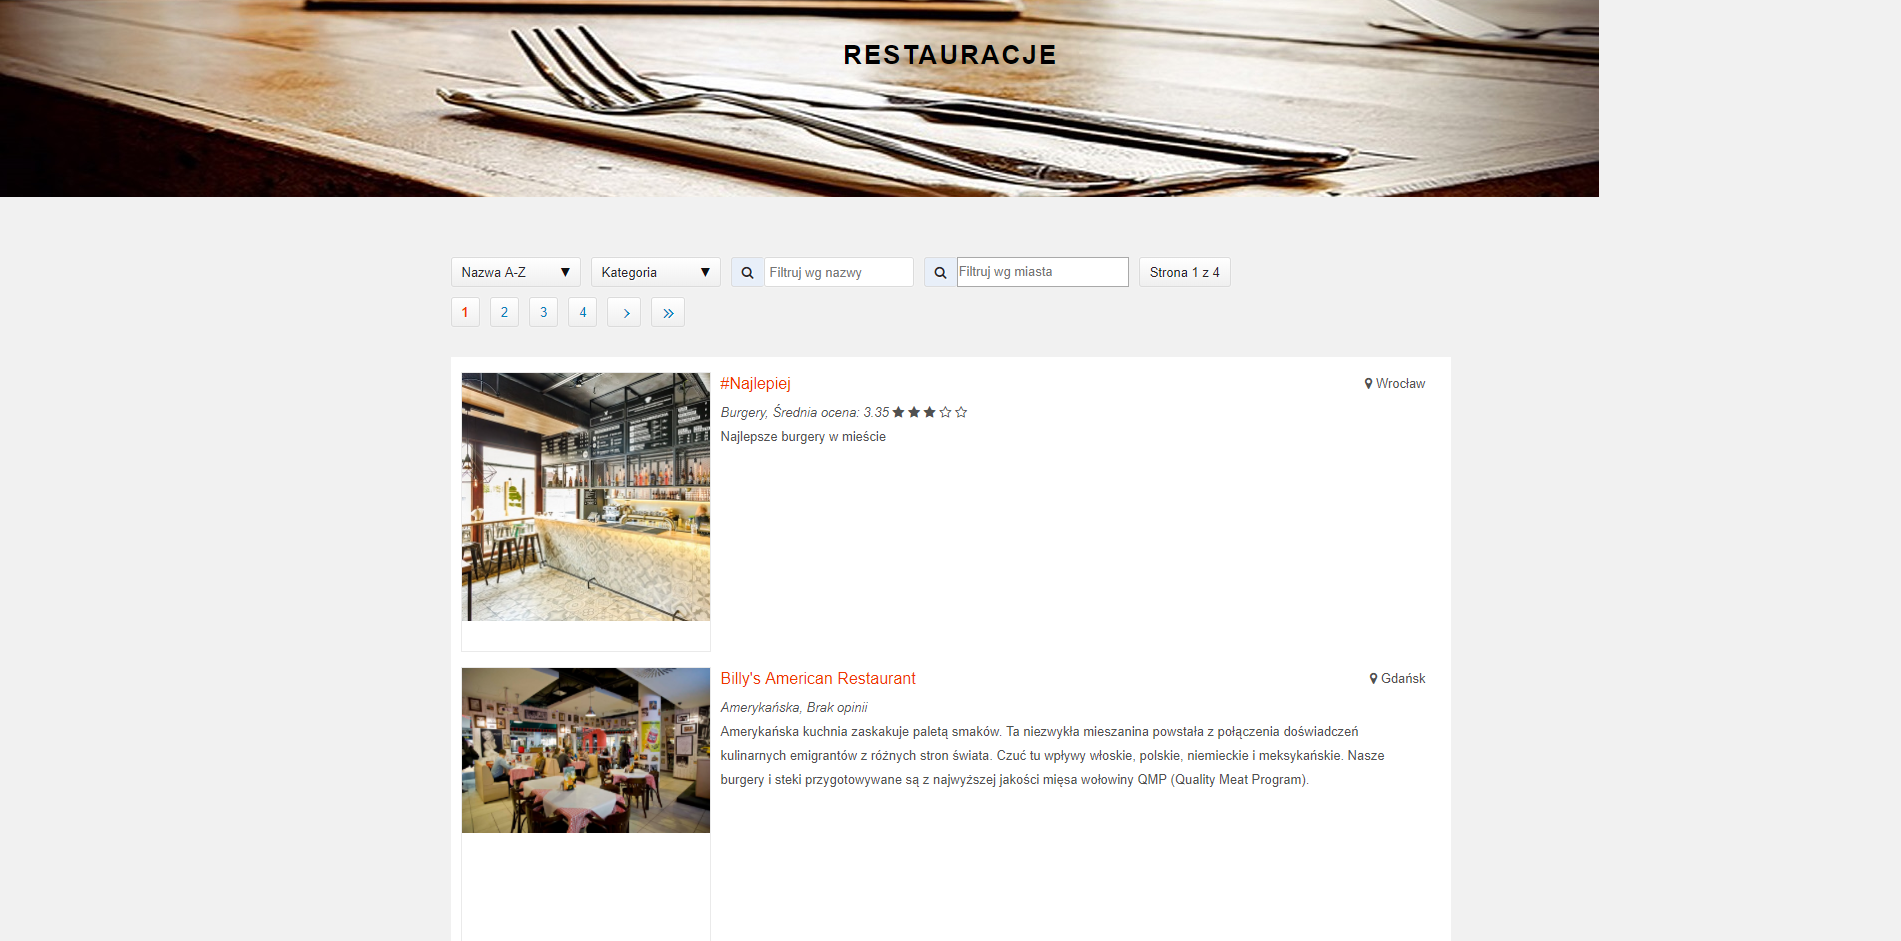
\includegraphics[width=1.00\textwidth]{screens/restaurants.png}
	\caption[caption]{Widok dostępnych restauracji.}
	\label{fig:restaurants}
\end{figure}

\begin{figure}[H]
\centering
	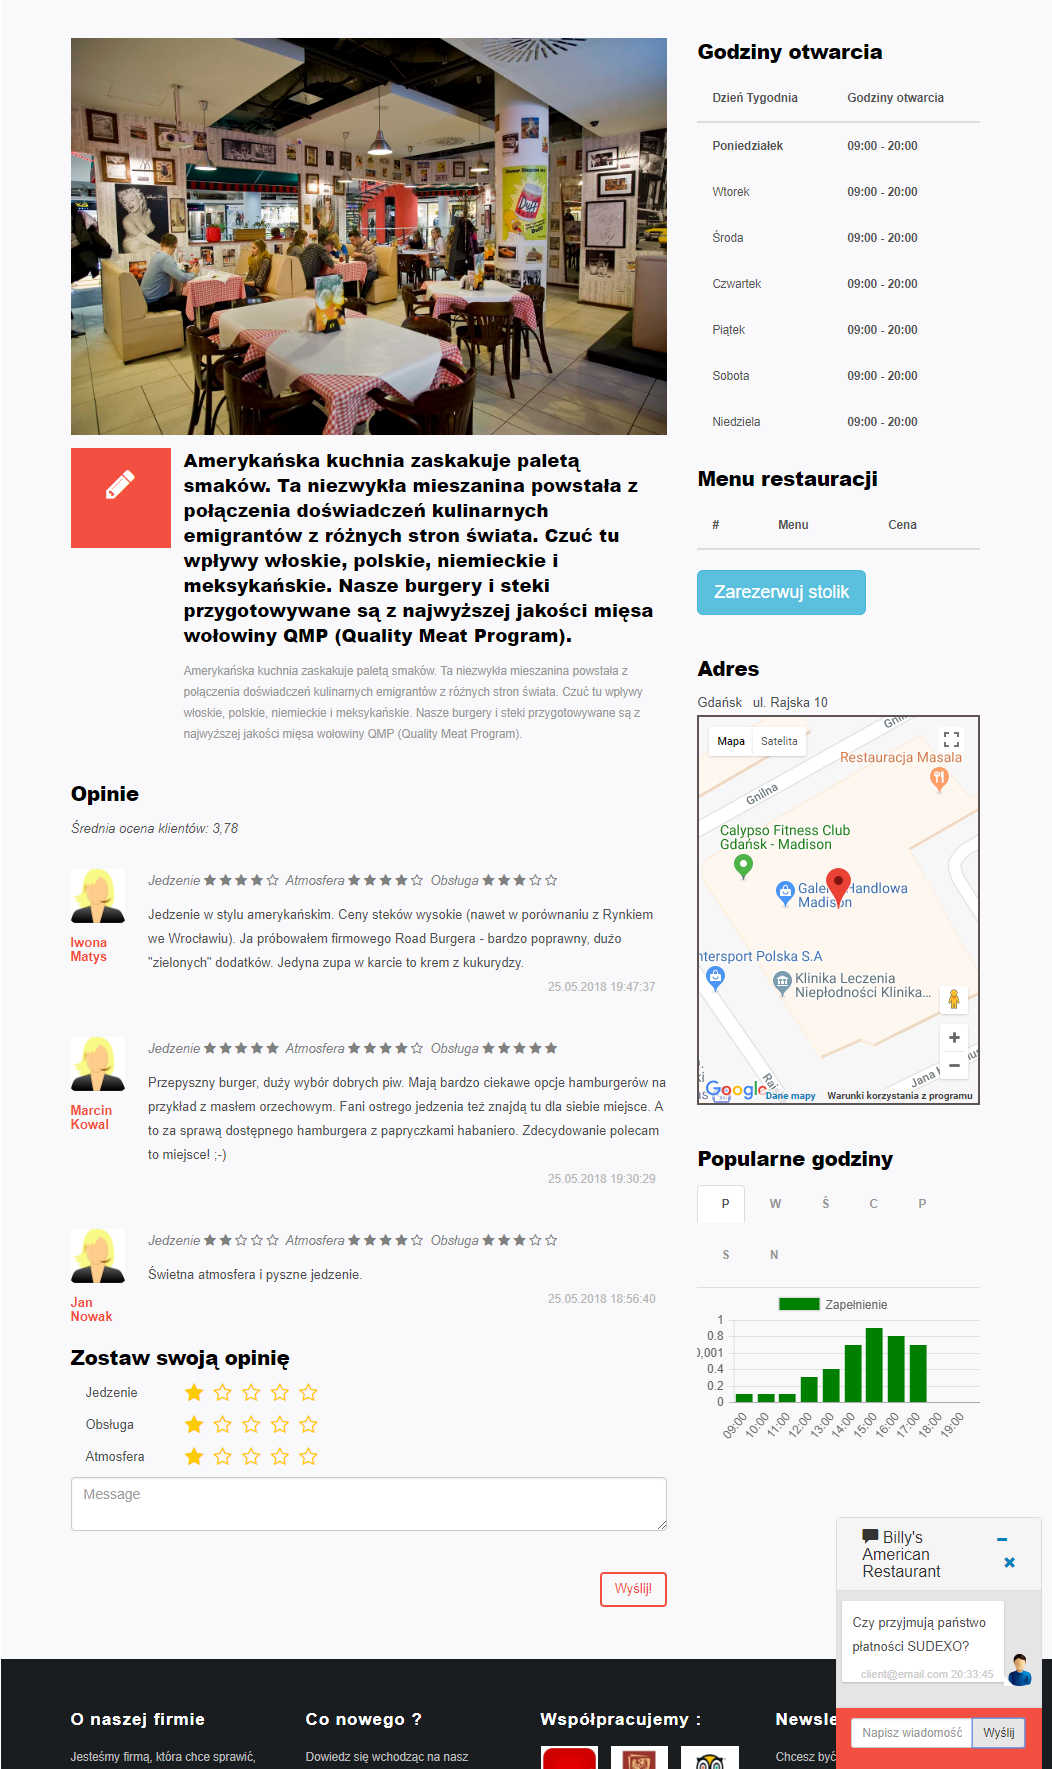
\includegraphics[width=1.00\textwidth]{screens/restaurant.png}
	\caption[caption]{Widok restauracji.}
	\label{fig:restaurant}
\end{figure}

\begin{figure}[H]
\centering
	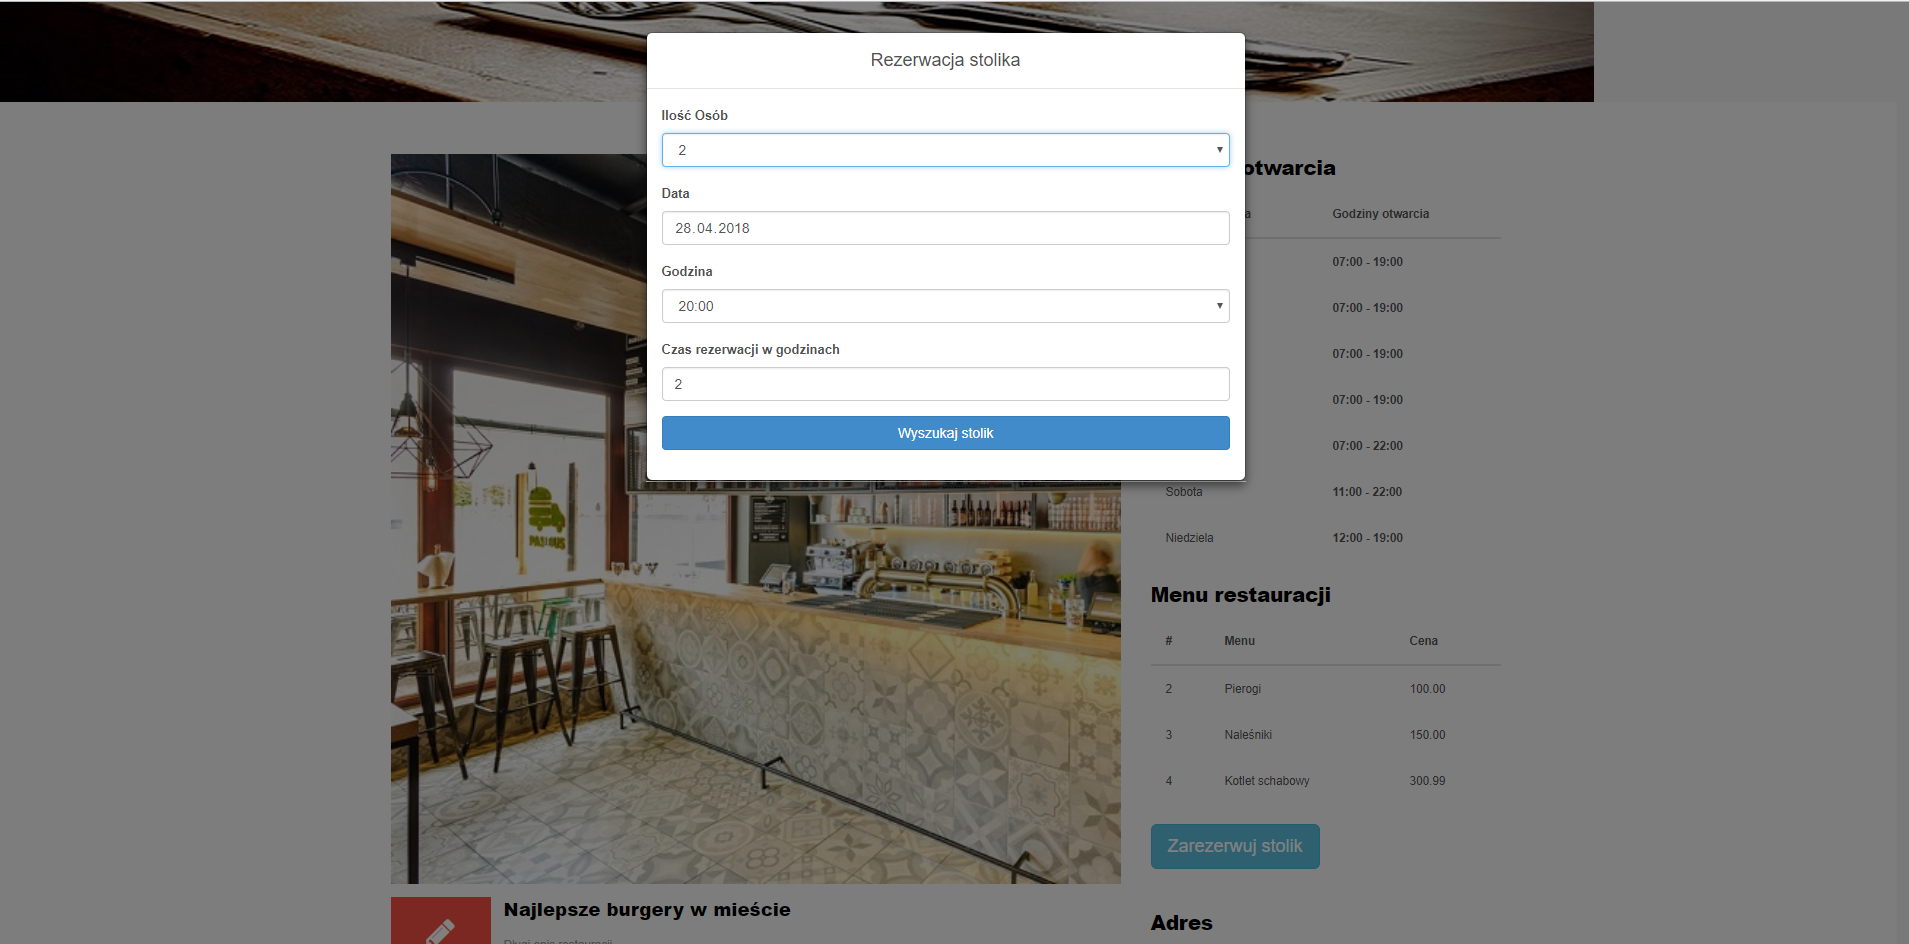
\includegraphics[width=1.00\textwidth]{screens/reservation.png}
	\caption[caption]{Widok rezerwacji stolika.}
	\label{fig:reservation}
\end{figure}

Użytkownik może przeglądać dostępne restauracje w widoku restaurants, dostępnym przez przycisk w pasku nawigacyjnym "Restauracje". Po wybraniu restauracji użytkownik jest przekierowywany do widoku zawierającego szczegóły restauracji (ref. \ref{fig:restaurant}). Widok zawiera godziny otwarcia rezerwacji, opinie innych użytkowników, dane restauracji, opis, popularne godziny oraz chat. Użytkownik dokonuje rezerwacji przez naciśnięcie "Zarezerwuj stolik". W okienku należy wybrać ilość osób dla których ma zostać złożona rezerwacja, data rezerwacji, godzinę i czas trwania rezerwacji. Po wciśnięciu "Wyszukaj stolik" aplikacja sprawdza czy stoliki są dostępne w danym momencie i prezentuje dostępne kombinacje stolików w danych godzinach. Po zatwierdzeniu rezerwacji użytkownik otrzymuje maila ze szczegółami rezerwacji. Restaurator musi potwierdzić rezerwację, aby się odbyła.

\begin{figure}[H]
\centering
	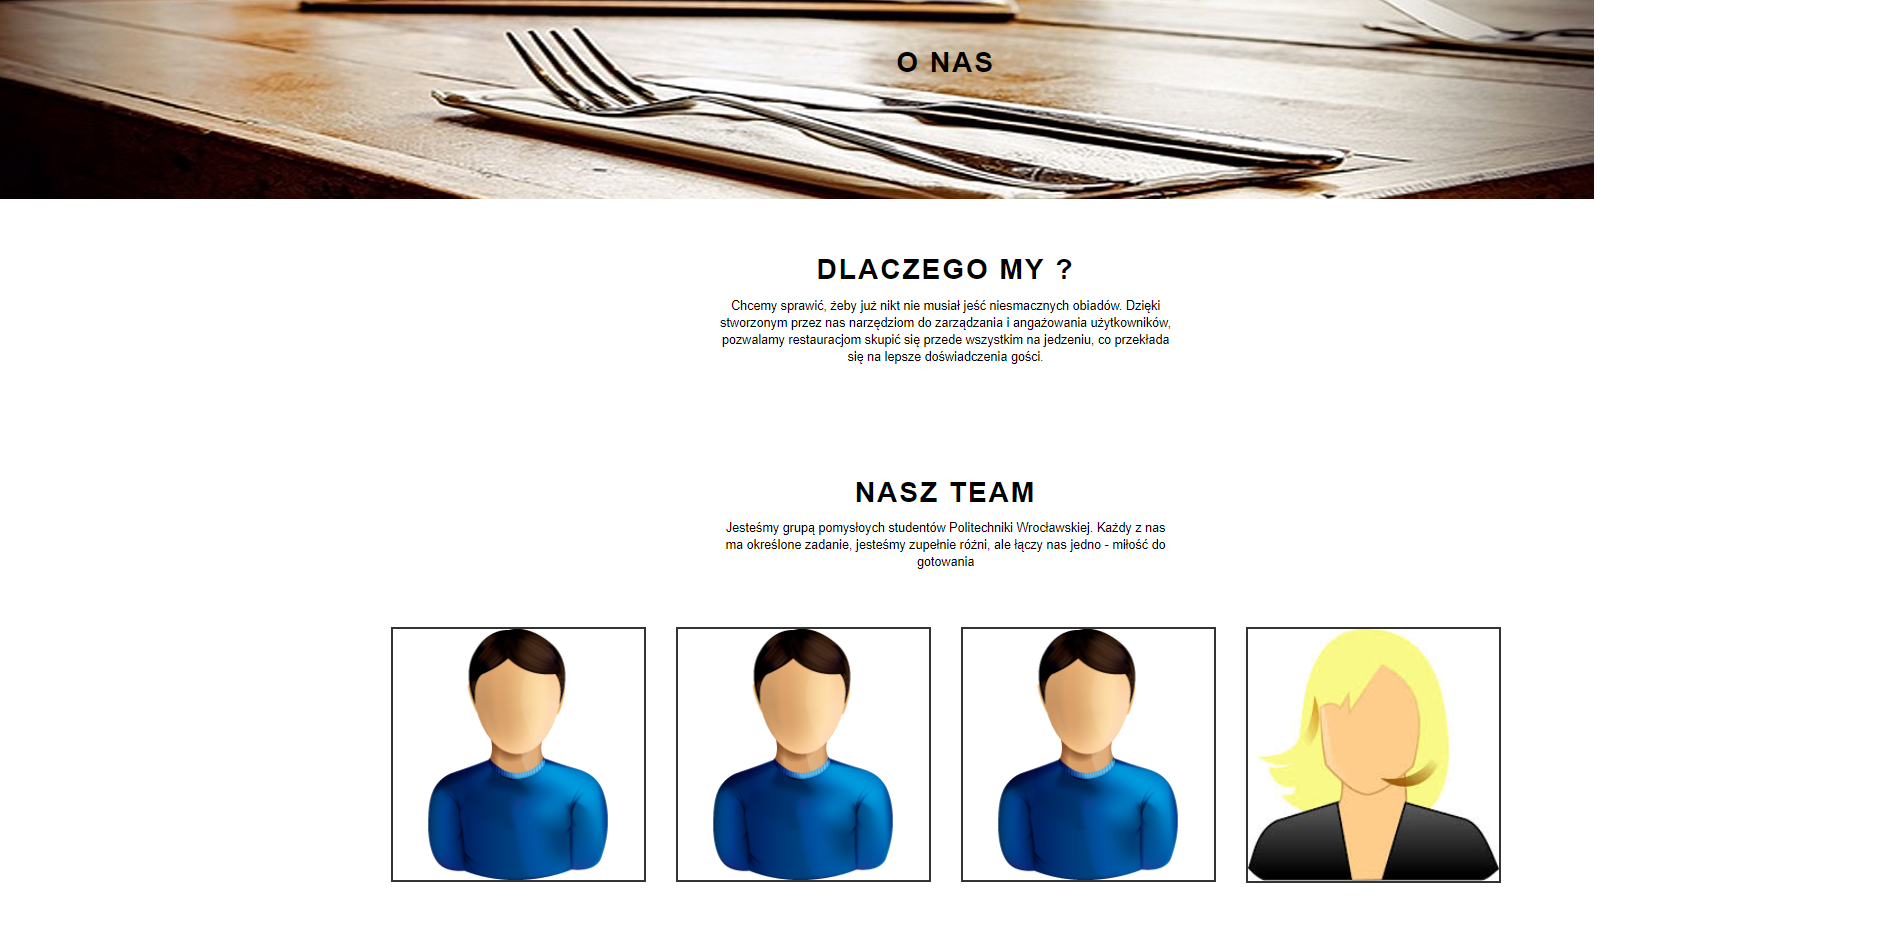
\includegraphics[width=1.00\textwidth]{screens/about.png}
	\caption[caption]{Widok zawierający informacje o zespole tworzącym aplikację.}
	\label{fig:about}
\end{figure}

\begin{figure}[H]
\centering
	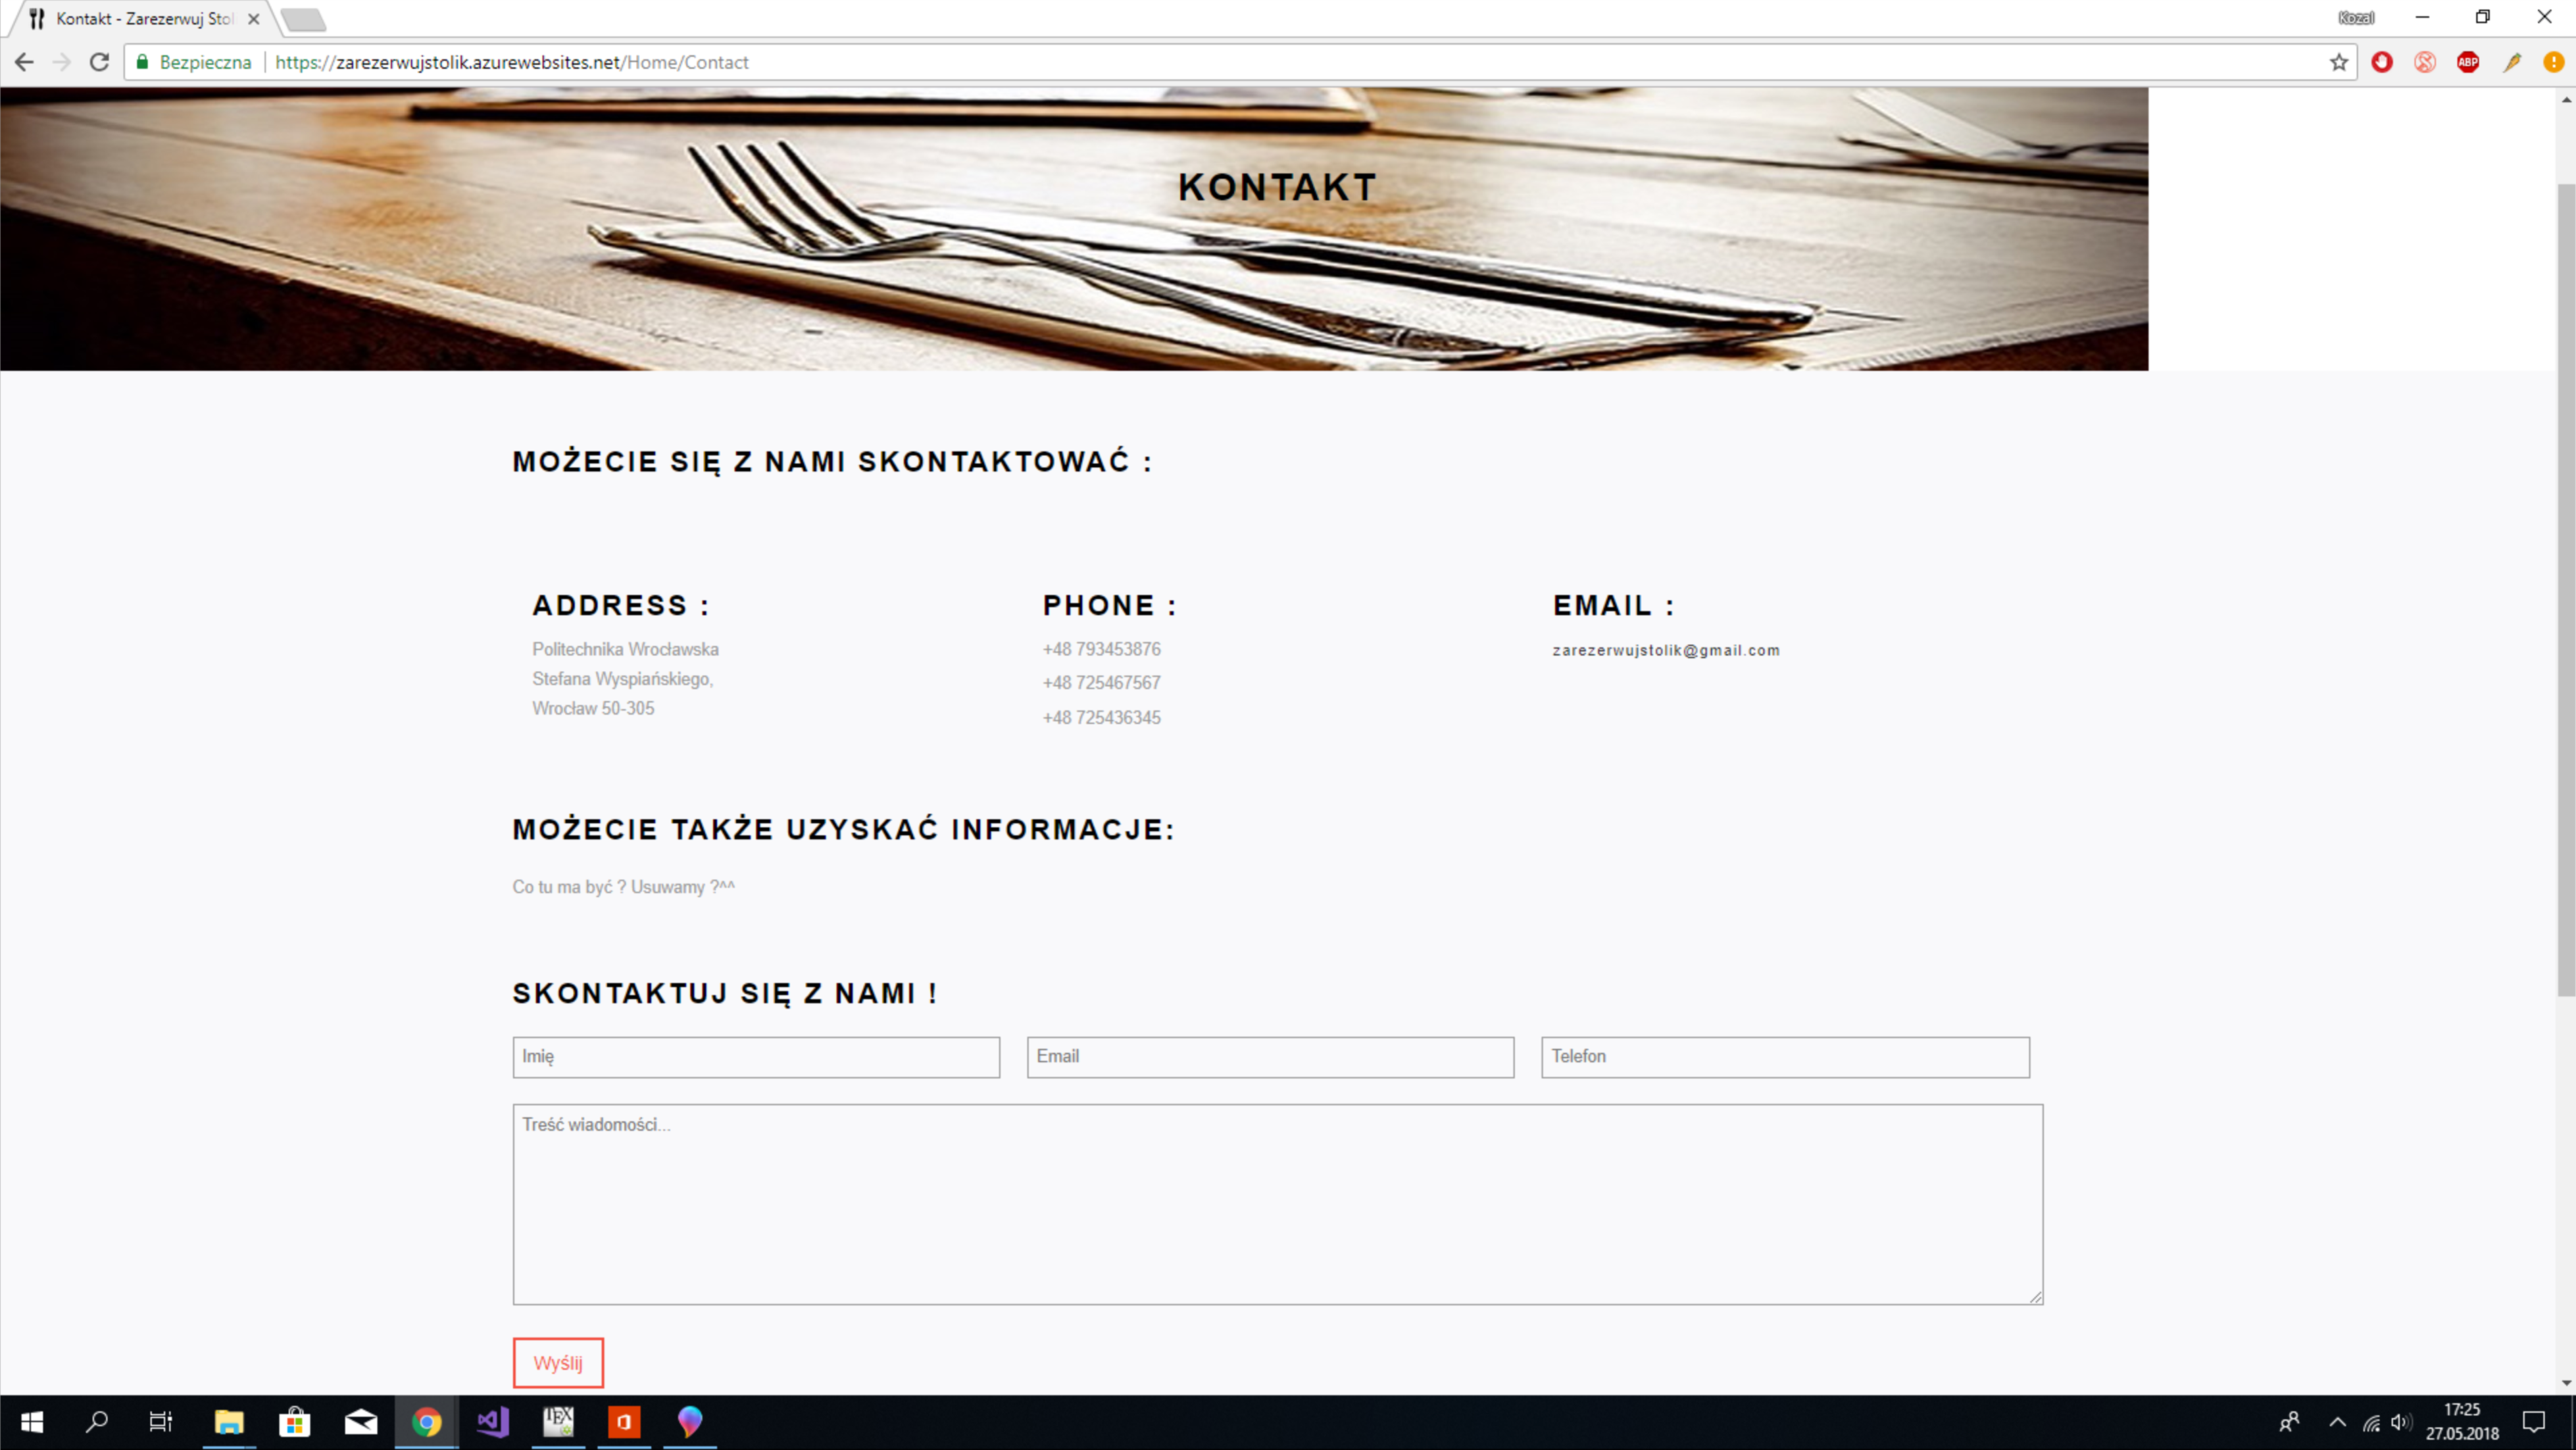
\includegraphics[width=1.00\textwidth]{screens/contact.png}
	\caption[caption]{Widok zawierający dane kontaktowe twórców aplikacji.}
	\label{fig:contact}
\end{figure}

Widoki dostępne po naciśnięciu w pasku nawigacyjnym przycisku "O nas", oraz "Kontakt" zawierają informacje na temat zespołu tworzącego aplikację (rys. \ref{fig:about}), oraz dane kontaktowe (rys. \ref{fig:contact}).

\begin{figure}[H]
\centering
	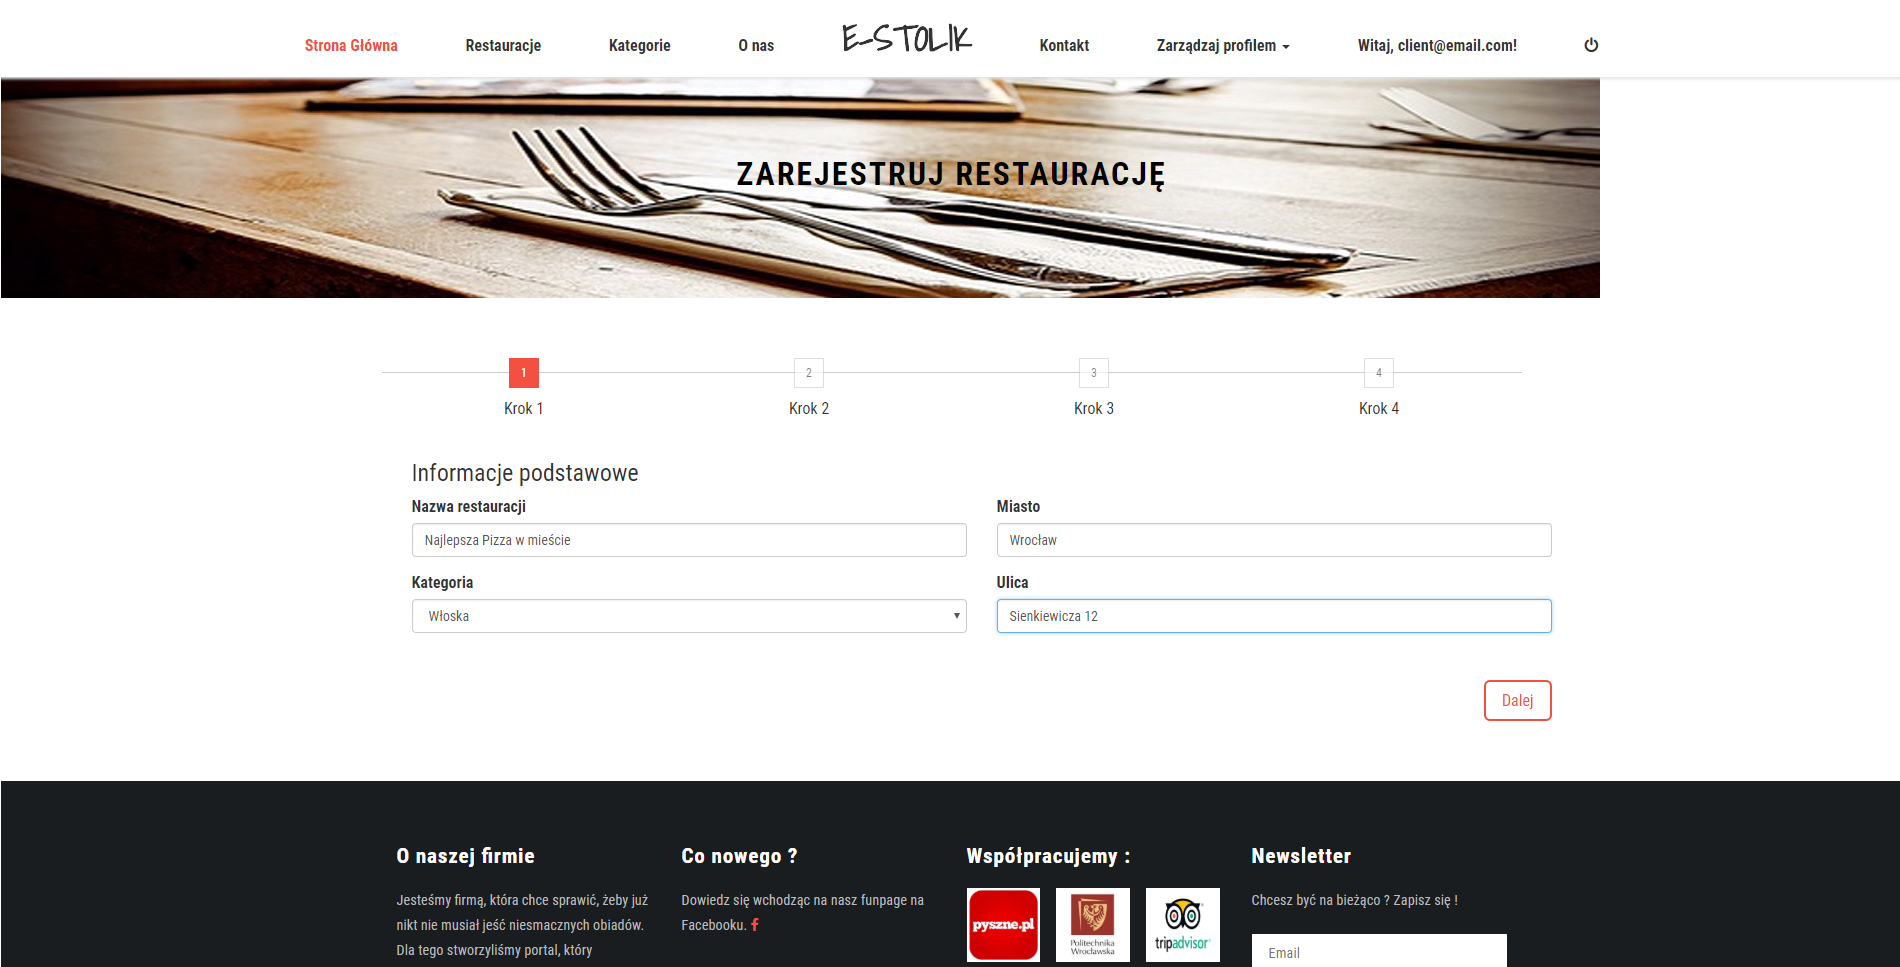
\includegraphics[width=1.00\textwidth]{screens/register_rest_1.png}
	\caption[caption]{Pierwszy krok rezerwacji restauracji.}
	\label{fig:register_rest_1}
\end{figure}

\begin{figure}[H]
\centering
	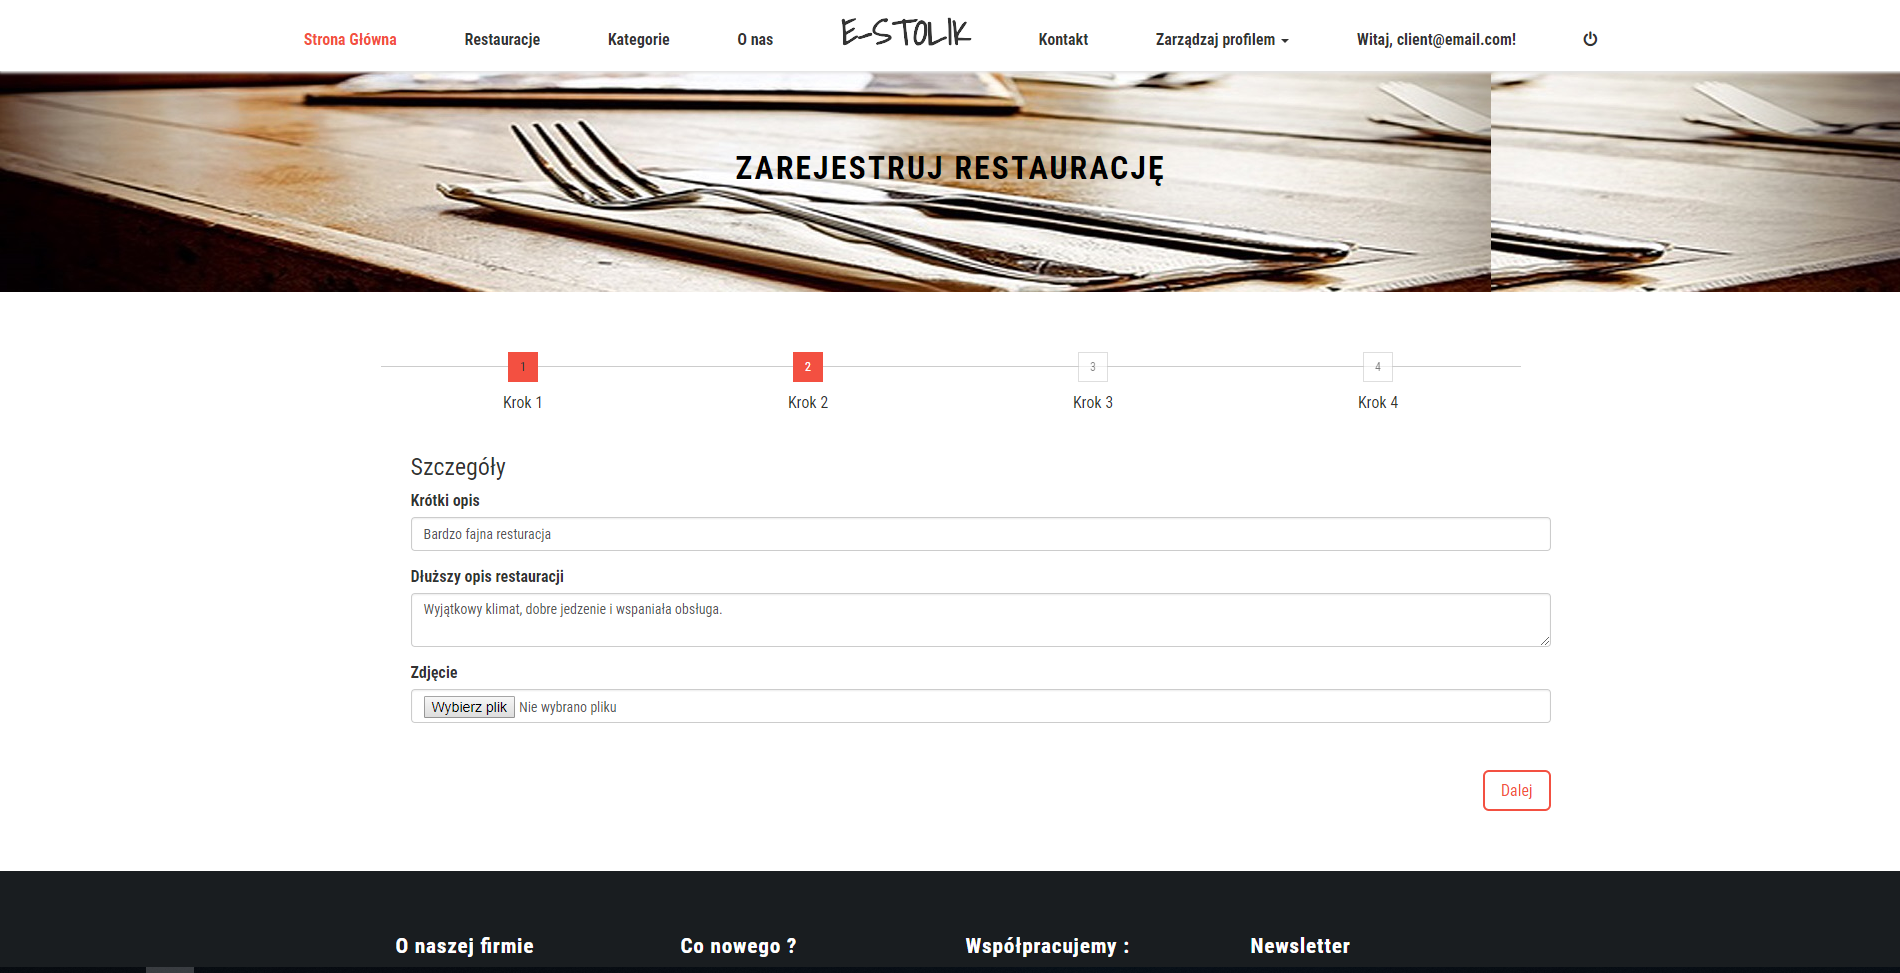
\includegraphics[width=1.00\textwidth]{screens/register_rest_2.png}
	\caption[caption]{Drugi krok rezerwacji restauracji.}
	\label{fig:register_rest_2}
\end{figure}

\begin{figure}[H]
\centering
	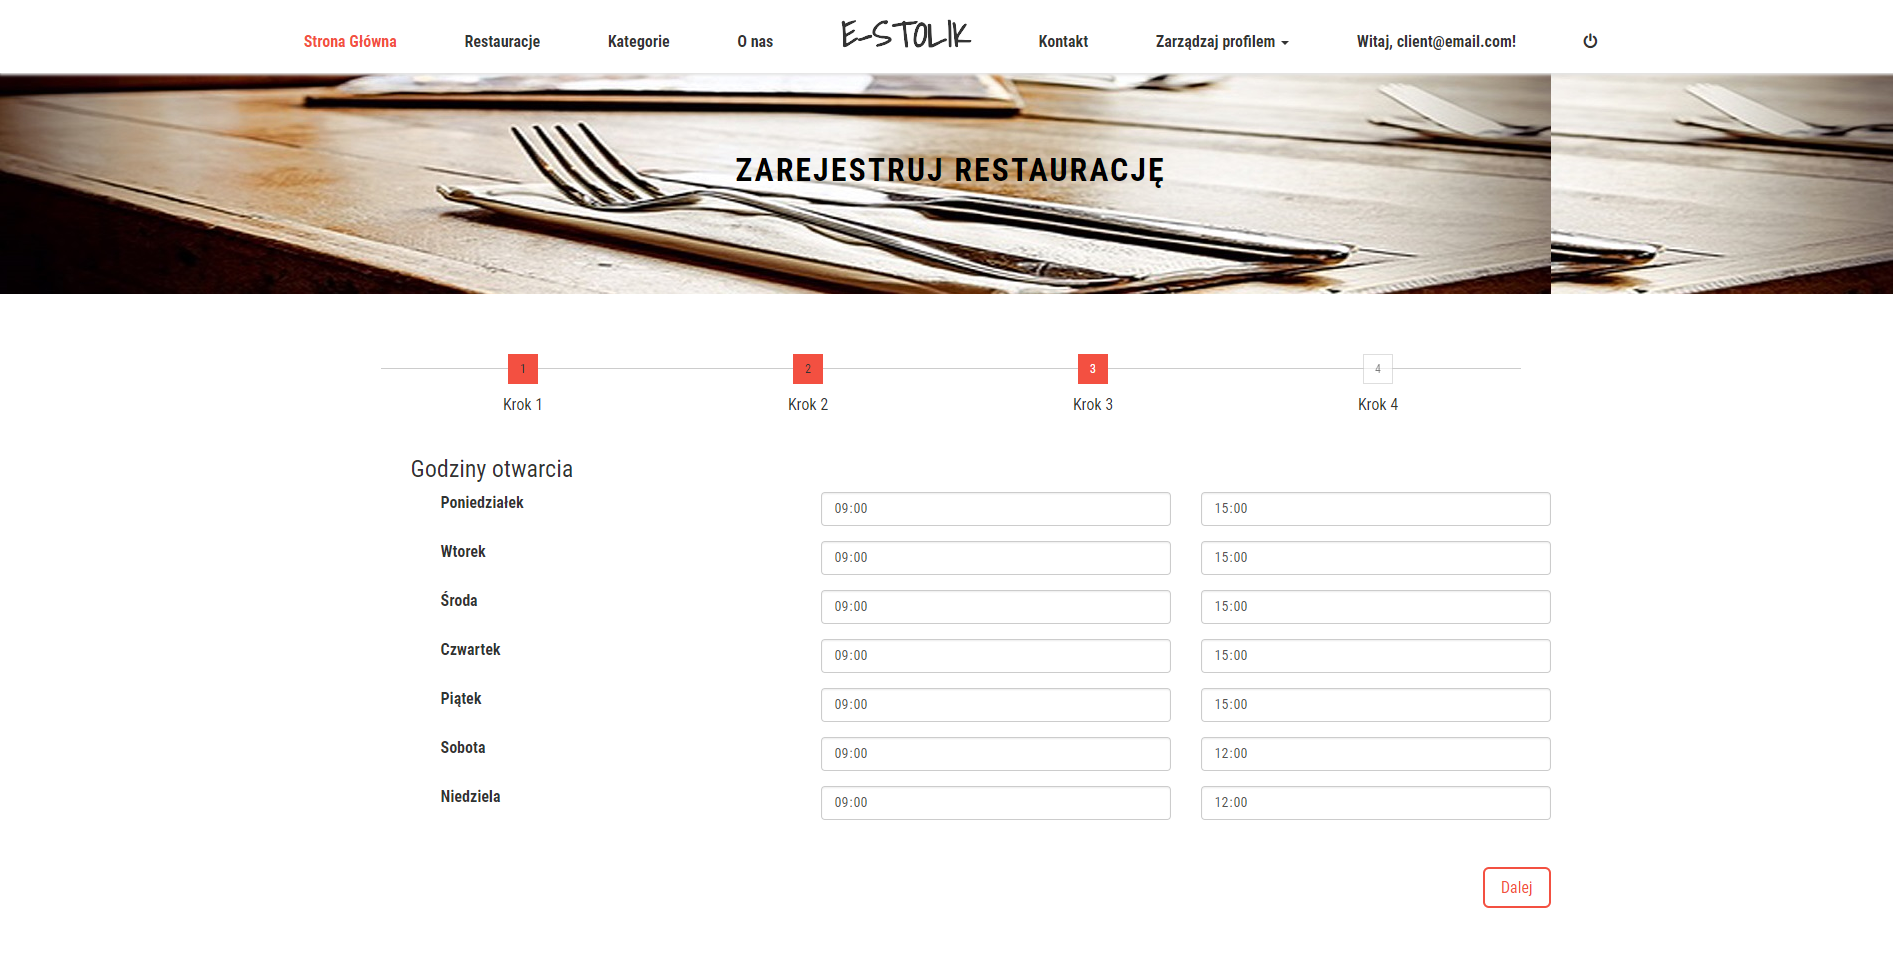
\includegraphics[width=1.00\textwidth]{screens/register_rest_3.png}
	\caption[caption]{Trzeci krok rezerwacji restauracji.}
	\label{fig:register_rest_3}
\end{figure}

\begin{figure}[H]
\centering
	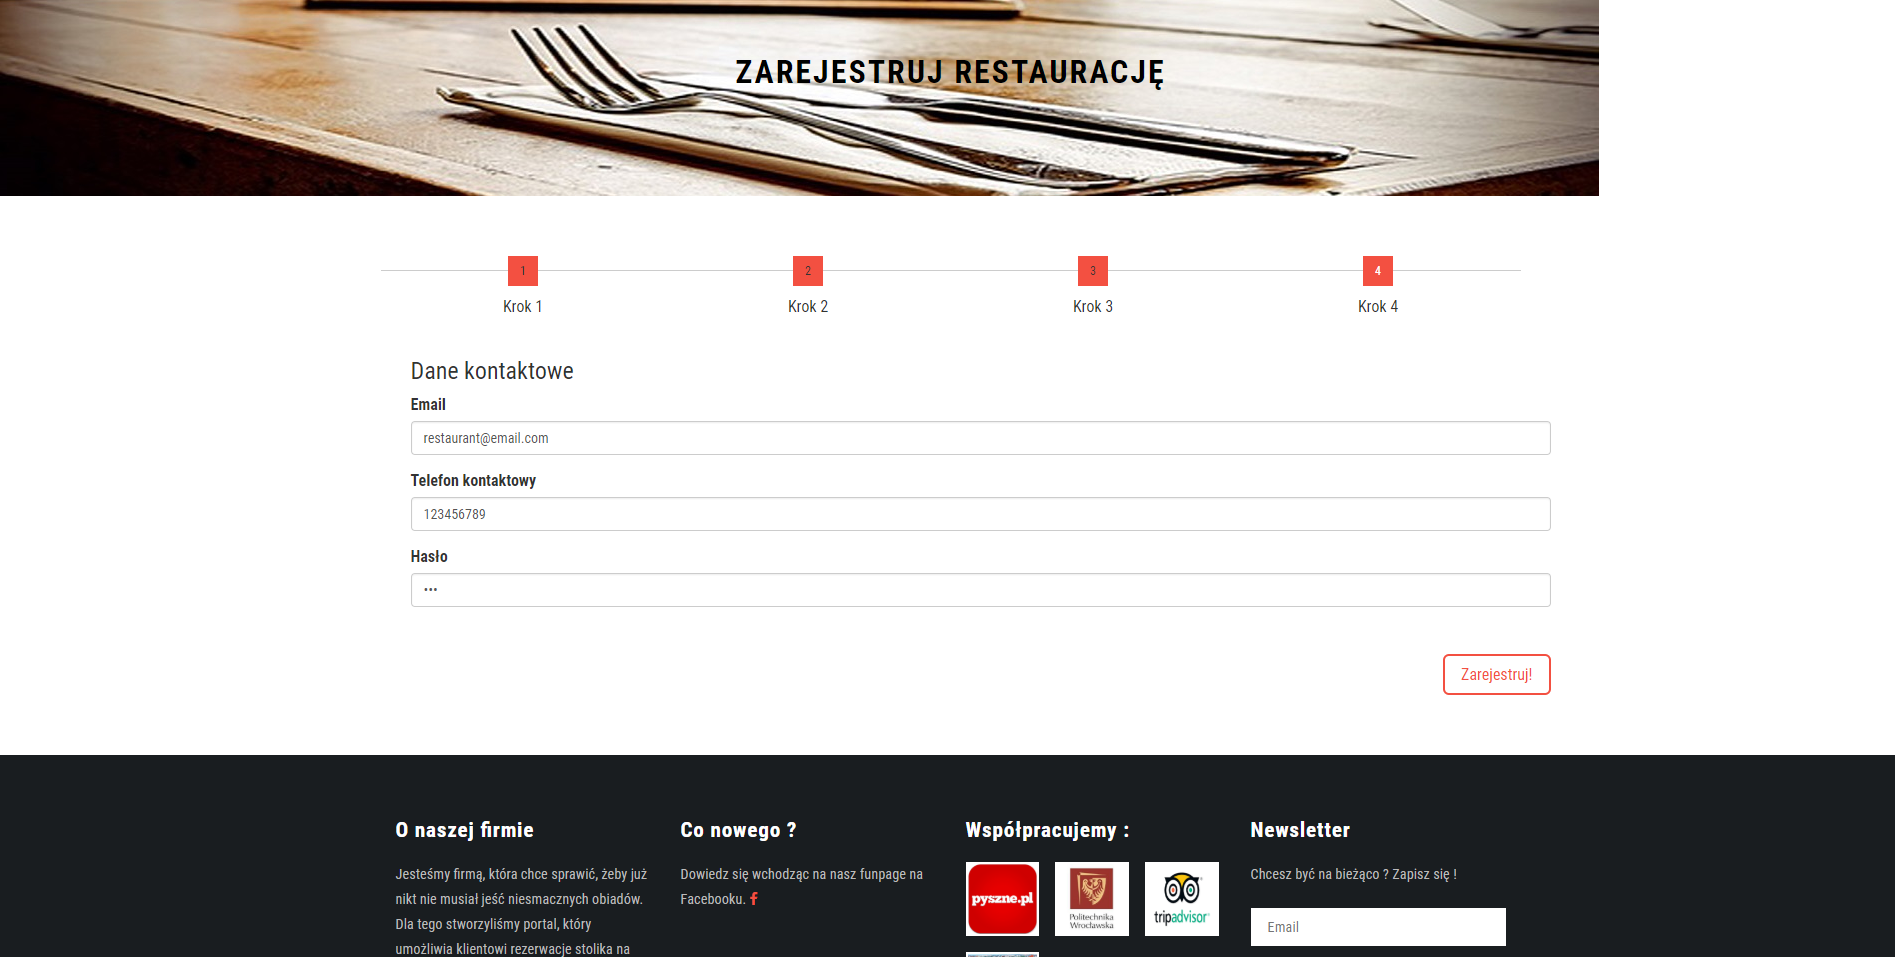
\includegraphics[width=1.00\textwidth]{screens/register_rest_4.png}
	\caption[caption]{Czwarty krok rezerwacji restauracji.}
	\label{fig:register_rest_4}
\end{figure}

Aby dokonać rejestracji restauracji (rys. \ref{fig:register_rest_1}-\ref{fig:register_rest_4}) należy podać kolejno: dane podstawowe, opisy restauracji, godziny otwarcia oraz mail, telefon i hasło do konta. Rejestracja jest dostępna na stronie głównej. W celu odfiltrowania fałszywych kont rejestracja restauracji musi być potwierdzona przez administratora systemu.

\subsection{Projekt bazy danych}
Aplikacja wykorzystuje dwie bazy danych. Jedna baza danych (rysunek \ref{fig:tier}) jest używana do zarządzania użytkownikami - dane logowania, ich role i inne dane potrzebne do weryfikacji. Tabele, jak i relacje w tej bazie danych zostały utworzone przy użyciu biblioteki ASP.NET Core Identity ze względu na szereg udostępnianych przez nią rozwiązań m.in. do logowania, rejestracji, przypominania czy resetowania haseł.
\begin{figure}[H]
\centering
	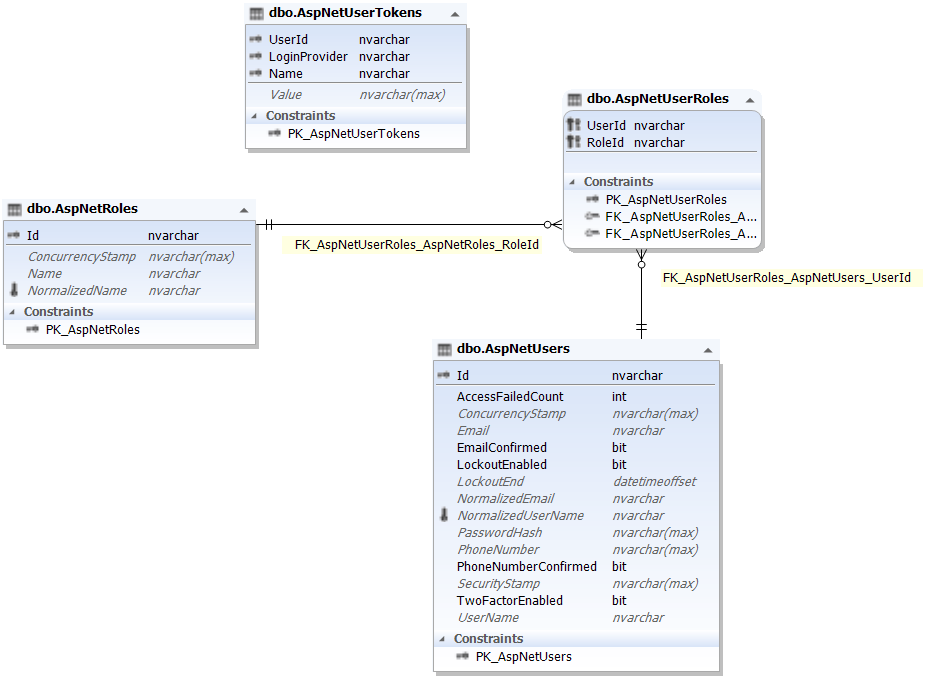
\includegraphics[width=0.90\textwidth]{bazaIdentity.png}
	\caption{Schemat bazy danych zarządzającej użytkownikami.}
	\label{fig:baza1}
\end{figure}
Drugą bazą danych jest baza zawierająca tabele potrzebne do obsługi aplikacji. Baza danych \ref{fig:baza2} jest powiązana przez unikalne pole \textit{IdentityId} w tabeli \textit{Customers/Restaurants} z polem Email w bazie danych \ref{fig:baza1}.
\begin{figure}[H]
\centering
	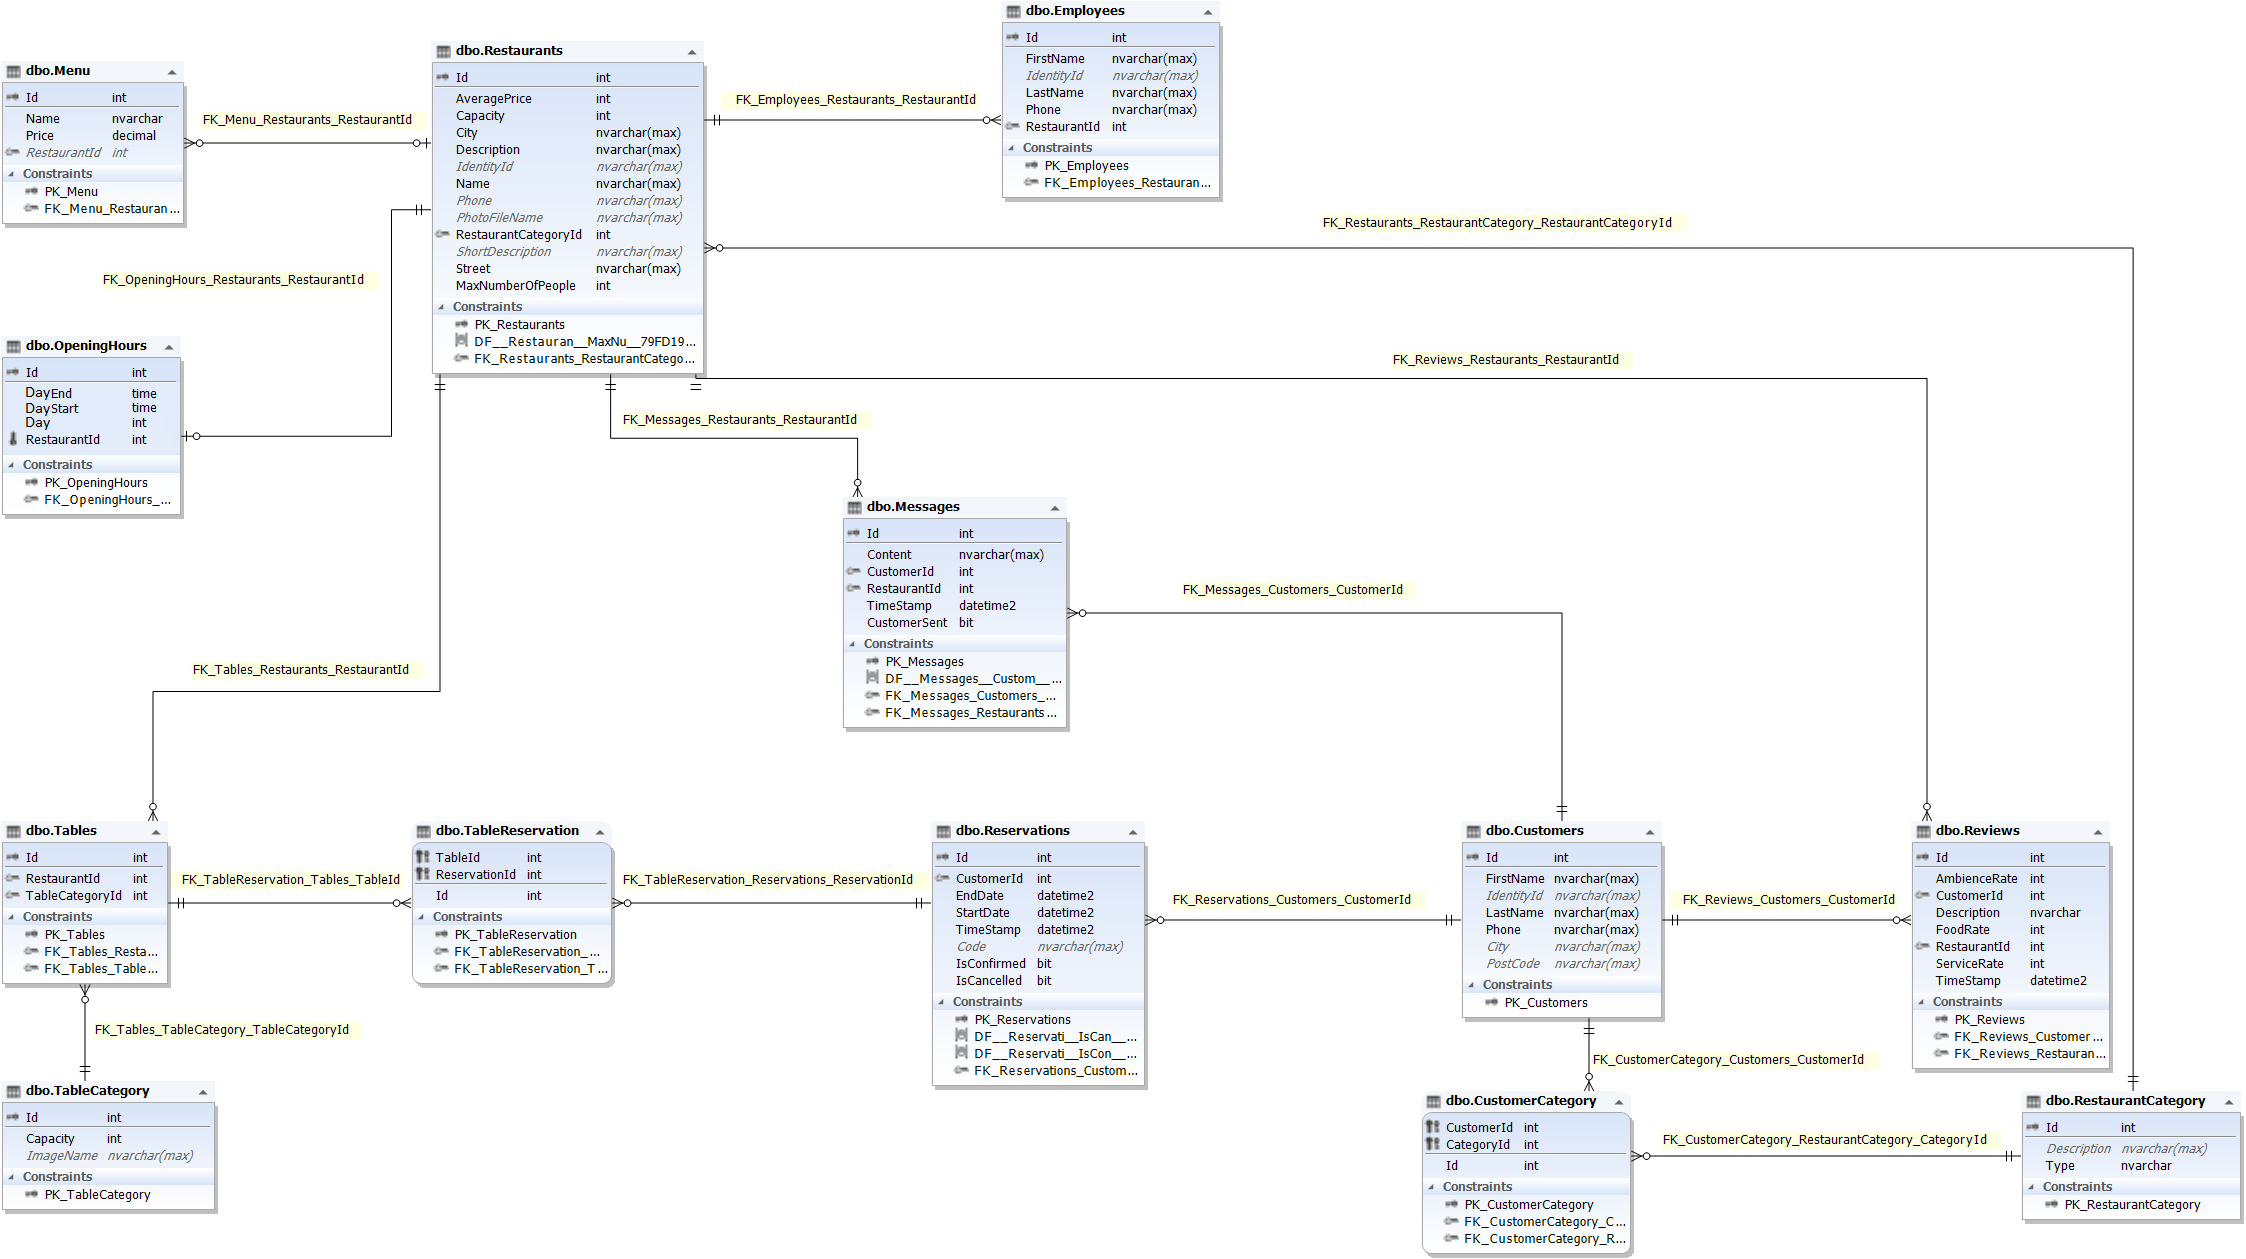
\includegraphics[angle=90,origin=c,width=\textwidth]{bazaStolik.png}
	\caption{Schemat bazy danych aplikacji.}
	\label{fig:baza2}
\end{figure}

\newpage
\subsection{Algorytm wyszukiwania stolików}
W trakcie składania zamówienia użytkownik aplikacji podaje liczbę osób, dla których mają zostać zarezerwowane miejsca. W celu określenia czy złożenie zamówienia w wybranych godzinach jest możliwe opracowano algorytm, tworzący kombinację stolików dostępnych w wybranym czasie. Wejście algorytmu stanowią:
idRestaracji,
ilość osób, dla których ma zostać zrealizowana rezerwacja,
godzina rozpoczęcia rezerwacji oraz
czas trwania rezerwacji.
Wyjście algorytmu stanowi lista kombinacji stolików dostępnych w wybranym czasie mogących pomieścić wszystkie osoby, dla których została zrealizowana rezerwacja. 

Przy projektowaniu algorytmu wykorzystano technikę dziel i rządź. Na każdym etapie dokonywano odcięć w celu podziału zadania na mniejsze i lepiej określone problemy.

\begin{figure}[h]
\centering
	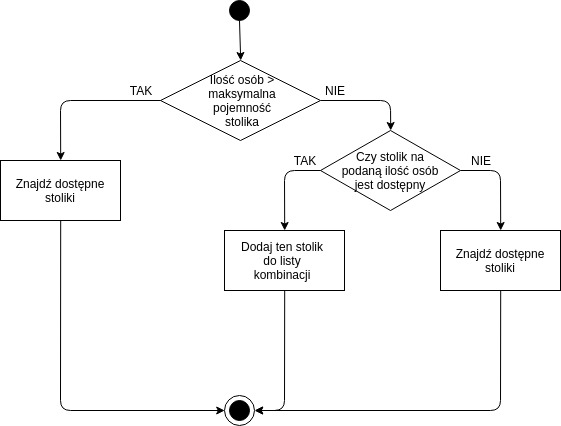
\includegraphics[width=0.70\textwidth]{algo1.jpg}
	\caption[caption]{Pierwszy krok działania algorytmu}
	\label{fig:alg1}
\end{figure}

Algorytm w pierwszym kroku (rys. \ref{fig:alg1}) określa czy podana w rezerwacji ilość osób może zostać posadzona przy jednym stoliku. Jeśli tak, sprawdzane jest czy stoliki o pojemności określonej równej ilości osób z rezerwacji są dostępne w wybranym czasie. Jeśli są dostępne algorytm kończy działanie i zwraca znaleziony stolik. Jeśli stolik nie jest dostępny, możliwe jest uzyskanie odpowiedniej ilości miejsc poprzez zajęcie mniejszych stolików (przykładem może być zarezerwowanie dwóch dwuosobowych stolików dla czterech osób). Odpowiedzialna jest za to procedura \textit{Znajdź dostępne stoliki} opisana poniżej. Procedura ta jest także wywoływana w przypadku gdy ilość osób w zamówieniu jest większa od stolika z największą pojemnością.

\begin{figure}[H]
\centering
	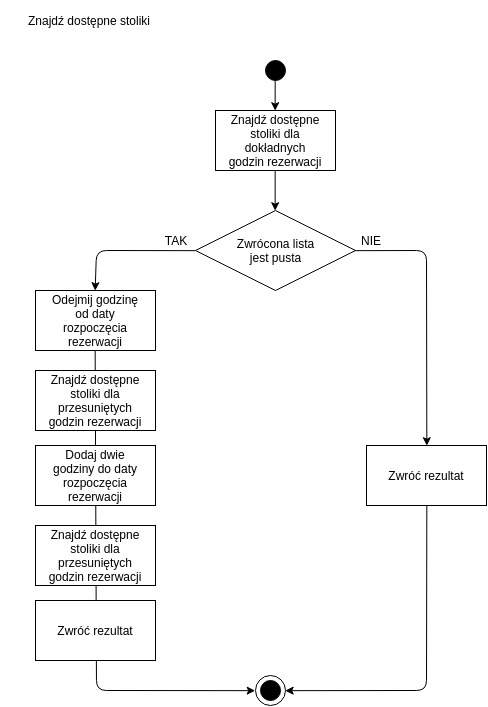
\includegraphics[width=0.50\textwidth]{algo2.jpg}
	\caption[caption]{Znajdź dostępne stoliki}
	\label{fig:alg2}
\end{figure}

Procedura \textit{Znajdź dostępne stoliki} określa czy są dostępne kombinacje stolików w podanych przez użytkownika godziny (rys. \ref{fig:alg2}). Jeśli zostanie znaleziona dowolna kombinacja będąca w stanie pomieścić ilość osób z rezerwacji procedura kończy działanie. W przeciwnym wypadku procedura modyfikuje godziny rozpoczęcia rezerwacji - dodaje i odejmuje godzinę od oryginalnej godziny rozpoczęcia rezerwacji i szuka kombinacji dla zmodyfikowanych dat.


\begin{figure}[H]
\centering
	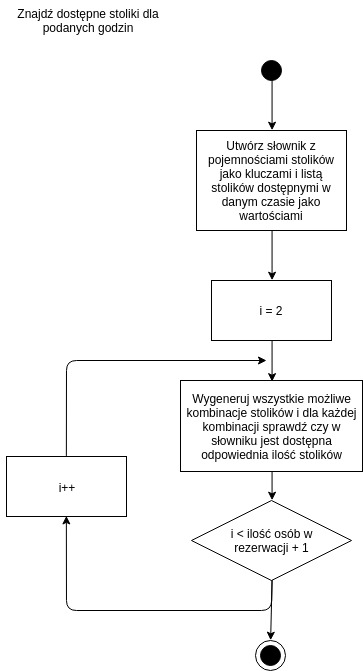
\includegraphics[width=0.50\textwidth]{algo3.jpg}
	\caption[caption]{Znajdź dostępne stoliki dla podanych godzin}
	\label{fig:alg3}
\end{figure}

Faktyczne szukanie kombinacji (rys. \ref{fig:alg3}) odbywa się z wykorzystaniem słownika mapującego pojemność stolików na listę stolików dostępnych w danym czasie o danej pojemności. Następnie, iterując po ilości stolików wyznacza się wszystkie możliwe kombinacje stolików (np. realizując zamówienie dla 10 osób przy użyciu dwóch stolików następujące kombinacje mogą zostać użyte dla zrealizowania zamówienia: \{\{8,2\},\{7,3\},\{6,4\},\{5,5\}\}). Dla wyznaczonej kombinacji sprawdza się, czy słownik zawiera odpowiednią ilość stolików dostępnych w danym czasie. Jeśli istnieją wolne stoliki potrzebne do utworzenia danej kombinacji w słowniku, kombinacja zostaje dodana do listy rozwiązań.

\section{Kamienie milowe i plan projektu}
\subsection{Wykres Gantta}

\begin{figure}[h]
\centering
	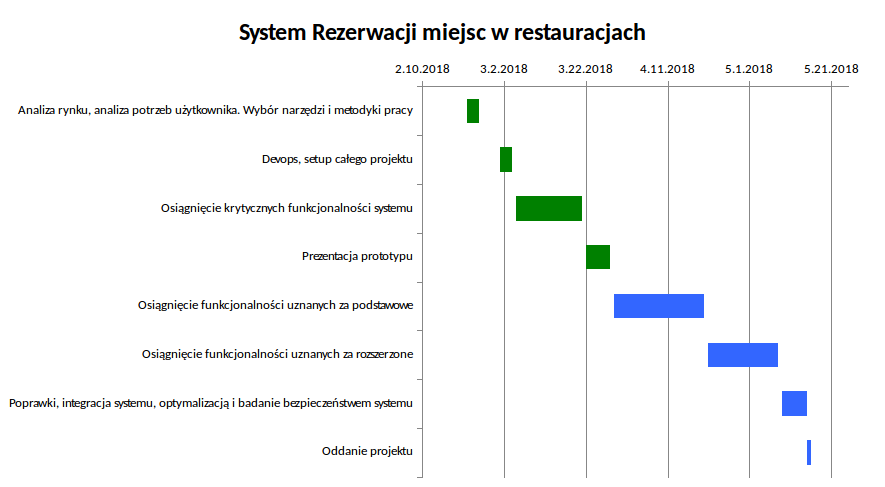
\includegraphics[width=0.70\textwidth]{gantt.png}
	\caption[caption]{Wykres Gantta.}
	\label{fig:gantt}
\end{figure}

Na rys. \ref{fig:gantt} przedstawiono wykres Gantta opracowany przed przystąpieniem do pracy nad projektem. Niestety przy opracowaniu tego wykresu poczyniono zbyt optymistyczne założenia, przez co nie udało się zrealizować planu przestawionego na wykresie.

\begin{figure}[h]
\centering
	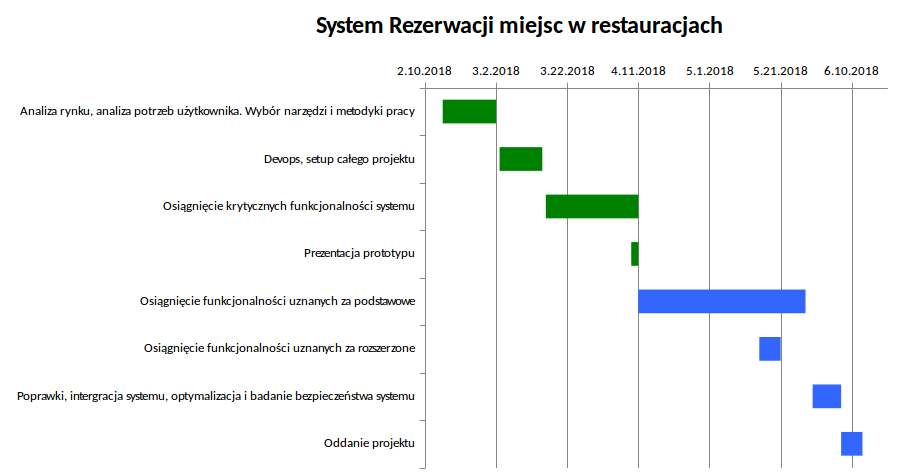
\includegraphics[width=0.70\textwidth]{gantt_real.png}
	\caption[caption]{Rzeczywisty wykres Gantta.}
	\label{fig:gantt}
\end{figure}

Na rys. \ref{fig:gantt} przedstawiono rzeczywisty wykres Gantta. Na osi czasu można zauważyć przesunięcie spowodowane wydłużeniem pracy nad krytycznymi oraz podstawowymi funkcjonalnościami systemu. Wszystkie opóźnienia spowodowały przesunięcie w czasie oddania projektu o około miesiąc.


\subsection{Rzeczywista kalkulacja kosztów i nakładów pracy}

Przed przystąpieniem do pracy nad projektem oszacowano koszta projektu uwzględniając honorarium czteroosobowego zespołu w wielkości 25 złotych za godzinę, oraz ubezpieczenie i podatki. Jako czas poświęcony na projekt przez każdego członka zespołu przyjęto 90 godzin. Jest to ilość godzin przewidzianych dla tego kursu w karcie przedmiotu. W wyniku obliczeń uzyskano:

\hspace*{0.35cm} łączne wynagrodzenie: 9000 zł \\
\tab ubezpieczenie (20.81\%): 1872.9 zł \\
\tab koszt bezpośredni: 10872.9 zł \\
\tab koszt pośredni: 0 zł \\
\tab koszt całkowity: 10872.9 zł \\
\tab podatek VAT (23\%): 2500,767 zł \\
\tab łączny koszt projektu: 13373,667 zł

W wyniku opóźnień i błędnej estymacji czas poświęcony na realizację projektu zwiększył się do  godzin. Było to powodem wzrostów kosztu projektu. Poniżej umieszczono czas poświęcony na projekt przez członków grupy, oraz rzeczywiste koszta projektu (z uwzględnieniem tej samej stawki):

\hspace*{0.35cm} Eliza Mocek: 130h \\
\tab Piotr Monetwka: 100h \\
\tab Jędrzej Kozal: 80h \\
\tab Hubert Duś: 80h \\

\hspace*{0.35cm} łączne wynagrodzenie: 9750 zł \\
\tab ubezpieczenie (20.81\%): 1872.9 zł \\
\tab koszt bezpośredni: 11778.98 zł \\
\tab koszt pośredni: 0 zł \\
\tab koszt całkowity: 11778.98 zł \\
\tab podatek VAT (23\%): 2709,16 zł \\
\tab łączny koszt projektu: 14488,14 zł

Jak widać opóźnienia przyczyniły się do wzrostu łącznego kosztu projektu o ponad 1000 złotych. W związku z nierównym udziałem i nakładem pracy różnych członków projektu proponuje się uwzględnienie godzinowego nakładu pracy członków zespołu przy wystawianiu oceny za projekt.


\section{Wdrożenie projektu}
Aplikacja sieci Web jak i baza danych została wdrożona z użyciem usług Microsoft Azure. Utworzony został serwer SQL zawierający dwie bazy danych (pierwszy zawierający bazę danych użytkowników oraz ich uprawnienia, drugi zawierający pozostałe tabele) oraz serwer aplikacji. Od docelowego użytkownika wymagana jest przeglądarka z dostępem do internetu. Aplikacja webowa została przetestowana w przeglądarce Google Chrome wersji 65 oraz Microsoft Edge 41.
\subsection{Adres URL}
Aplikacja jest dostępna pod adresem:
\begin{center}
\textit{https://zarezerwujstolik.azurewebsites.net}
\end{center}
\subsection{Konta testowe}
Przygotowane zostały dwa konta testowe:\\\\
\textbf{Konto restauracji:}
\begin{center}
Nazwa użytkownika: restaurant@email.com Hasło: Password1!
\end{center}
\textbf{Konto klienta:}
\begin{center}
Nazwa użytkownika: client@email.com Hasło: Password1!
\end{center}


\section{Podsumowanie i wnioski}


\newpage
\begin{thebibliography}{9}

\bibitem{oficjalna strona}
Oficjalna strona ASP.NET MVC
\\\texttt{https://www.asp.net/mvc}

\bibitem{oficjalna dokumentacja}
Oficjalna dokumentacja ASP.NET MVC
\\\texttt{https://docs.microsoft.com/pl\-pl/aspnet/\#pivot\=core\&panel\=core\_overview}

\bibitem{organizacja projektu}
Mosh Hamedani
\textit{Should you split your ASP.NET MVC project into multiple projects?}.
\\\texttt{https://programmingwithmosh.com/csharp/should-you-split-your\\-asp-net-mvc-project-into-multiple-projects/}

\end{thebibliography}



\end{document}